\documentclass[10pt]{beamer}

\usetheme[progressbar=frametitle]{metropolis}
\usepackage{appendixnumberbeamer}

\usepackage{listings}
\usepackage[T1]{fontenc}
\usepackage[utf8]{inputenc}

\title{Diffusion of innovation \\ within an agent-based model: \\ Spinsons, independence and advertising}
\author{Maria Kowalczyk, Anna Szymanek, Patryk Wielopolski}
\institute{Wrocław Univeristy of Technology and Science}
\date{}

\begin{document}

\maketitle

\begin{frame}{Introduction and motivation}
	Diffusion of innovations is a theory that seeks to explain how, why, and at what rate new ideas and technology spread.
	
	\begin{figure}
		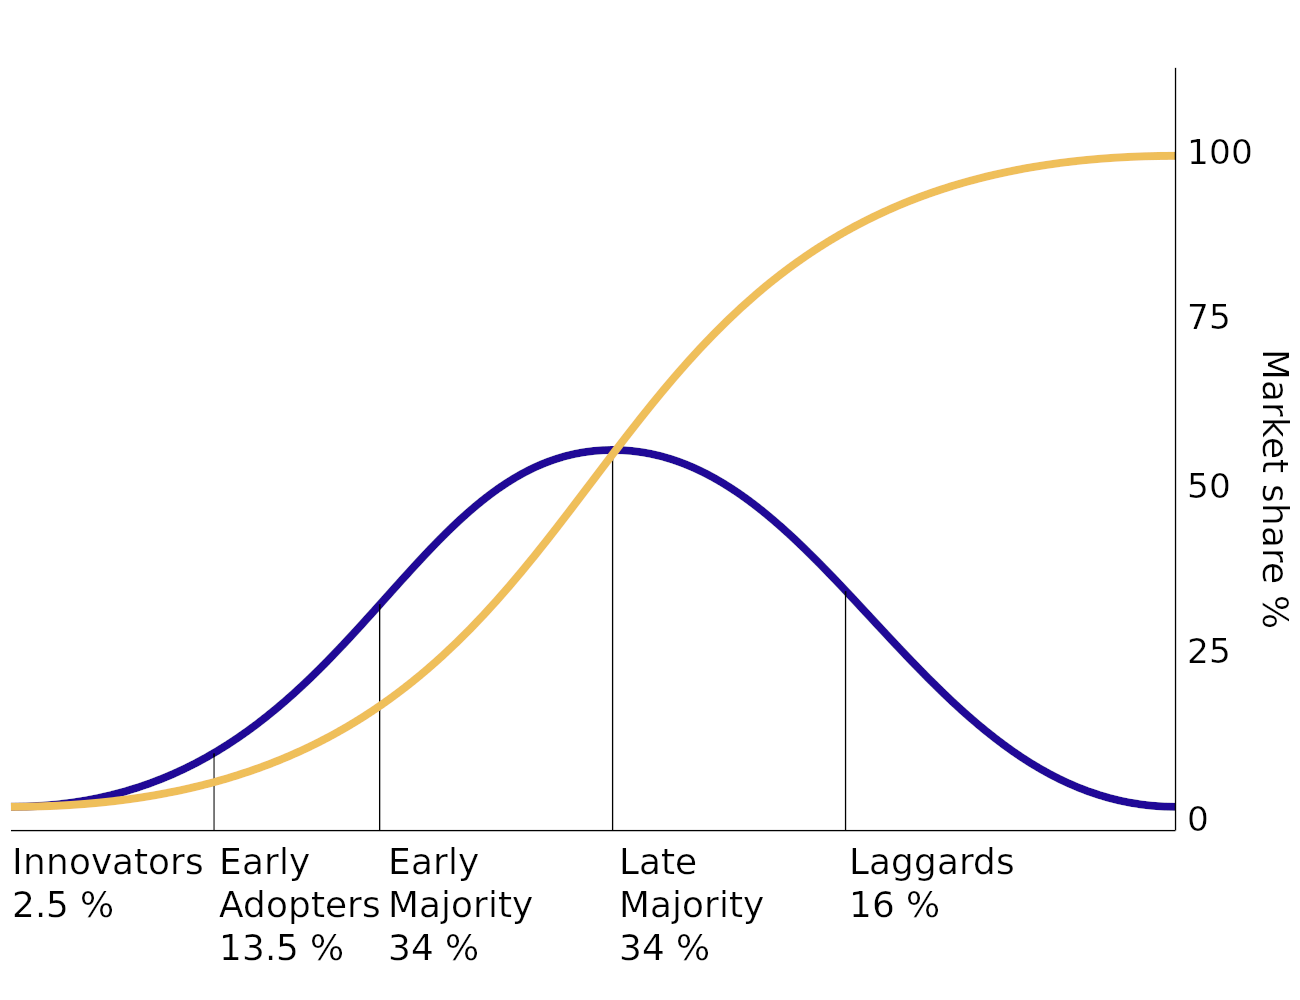
\includegraphics[height=0.5\textheight]{../resources/images/Diffusion_of_ideas.png}
		\caption{The diffusion of innovations according to E.Rogers. Source: \url{https://en.wikipedia.org/wiki/Diffusion\_of\_innovations\#/media/File:Diffusion\_of\_ideas.svg}}
	\end{figure}
	\nocite{article}
\end{frame}{}

\section{Diffusion of innovation model}

\begin{frame}{Model presentation}
	Model parameters
	\begin{itemize}
		\item Conformity $p$
		\item Independence $f$
		\item Advertising $h$
	\end{itemize}
\end{frame}

\begin{frame}{Conformity}
	\begin{figure}
		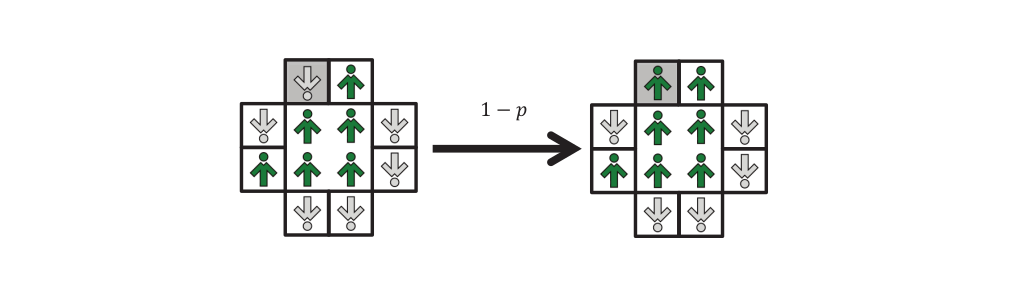
\includegraphics[width=\textwidth]{../resources/images/conformity.png}
		\caption{Schema of conformity $p$. Source: \cite{article}.}
	\end{figure}
\end{frame}

\begin{frame}{Independence}
	\begin{figure}
		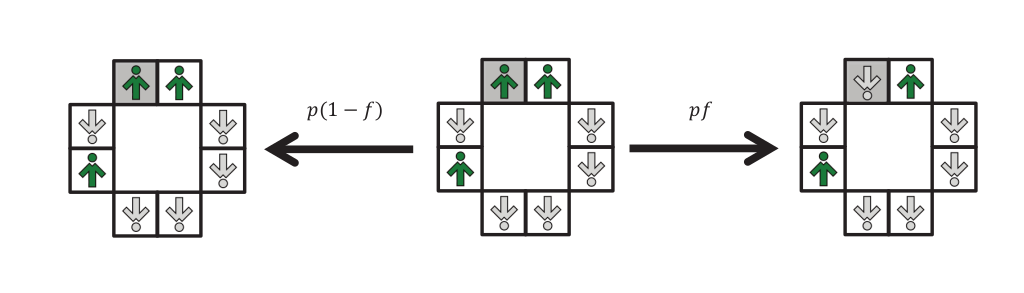
\includegraphics[width=\textwidth]{../resources/images/flexibility.png}
		\caption{Schema of independence $f$. Source: \cite{article}.}
	\end{figure}
\end{frame}

\begin{frame}{Advertising}
	\begin{figure}
		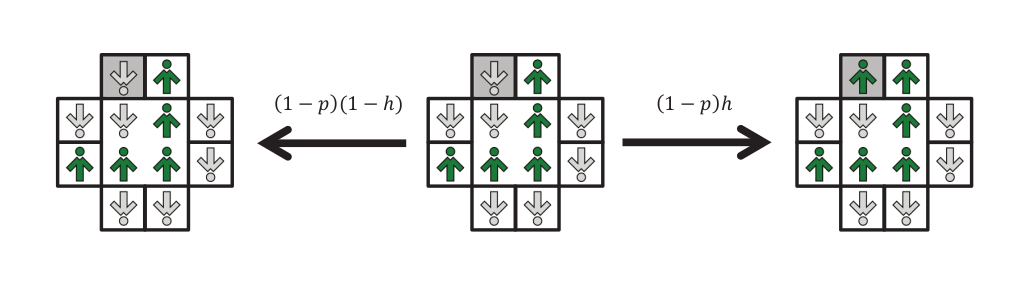
\includegraphics[width=\textwidth]{../resources/images/advertising.png}
		\caption{Schema of advertising $h$. Source: \cite{article}.}
	\end{figure}
\end{frame}

\begin{frame}{2D Lattice simulation}
	\begin{figure}
		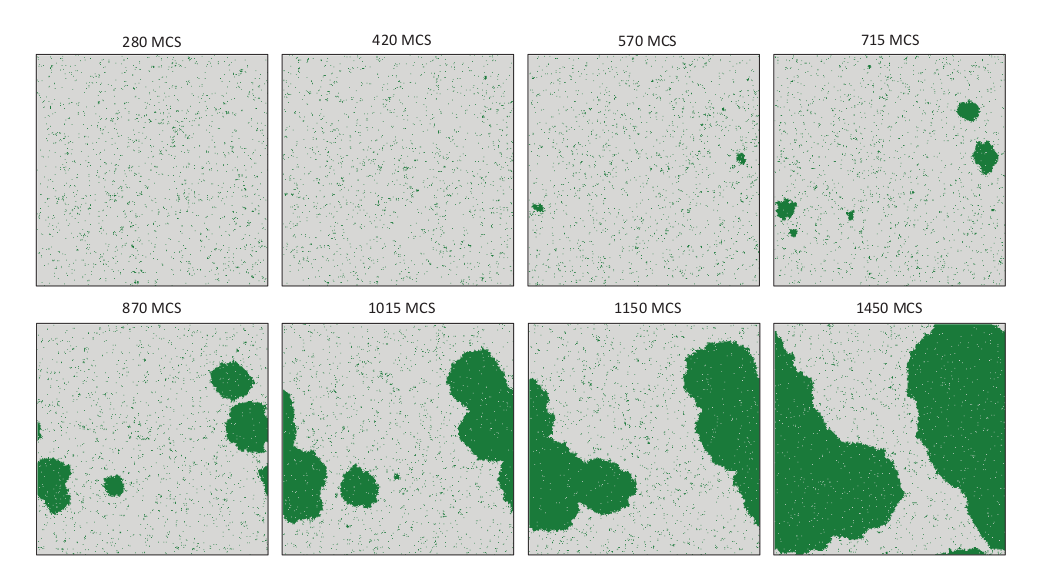
\includegraphics[height=0.4\textheight]{../resources/images/fig6.png}
		\hfill
		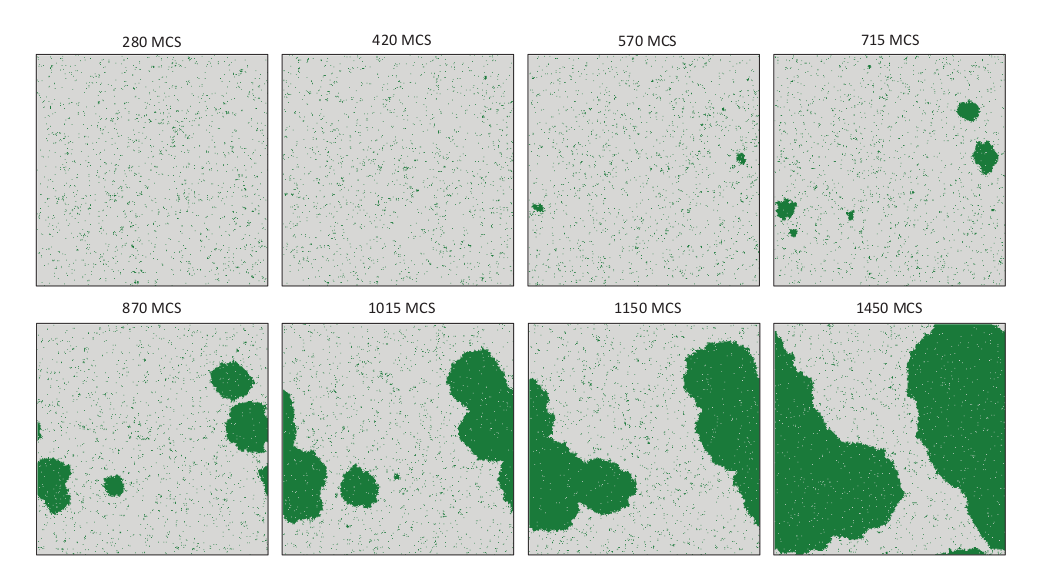
\includegraphics[height=0.4\textheight]{../resources/images/fig6.png}
		\caption{Up - publication; down - ours.}
	\end{figure}
\end{frame}

\section{Concentration in time}

\begin{frame}{Concentration}
	Concentration
	$$ c_t = \frac{N_{\uparrow}(t)}{N} $$ 
	where 
	\begin{itemize}
		\item $ N_{\uparrow}(t) $ - number of adopted people, i.e. spinsons with opinion = 1
		\item $ N $ - number of people in network
	\end{itemize}

\end{frame}

\begin{frame}{2D Lattice results}
	\begin{figure}
		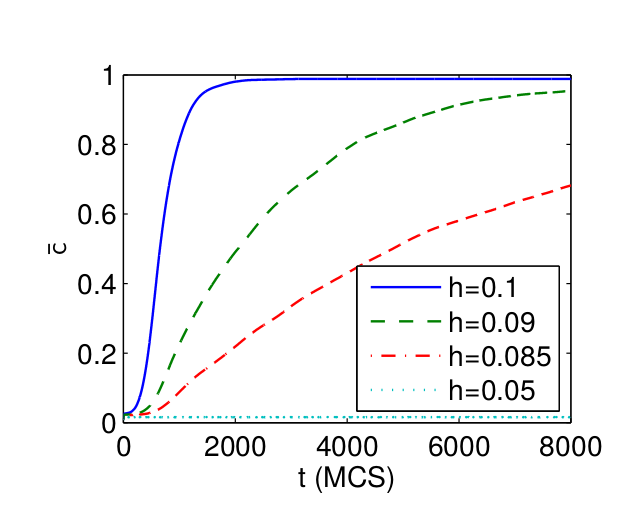
\includegraphics[width=0.475\textwidth]{../resources/images/fig7-left.png}
		\hfill
		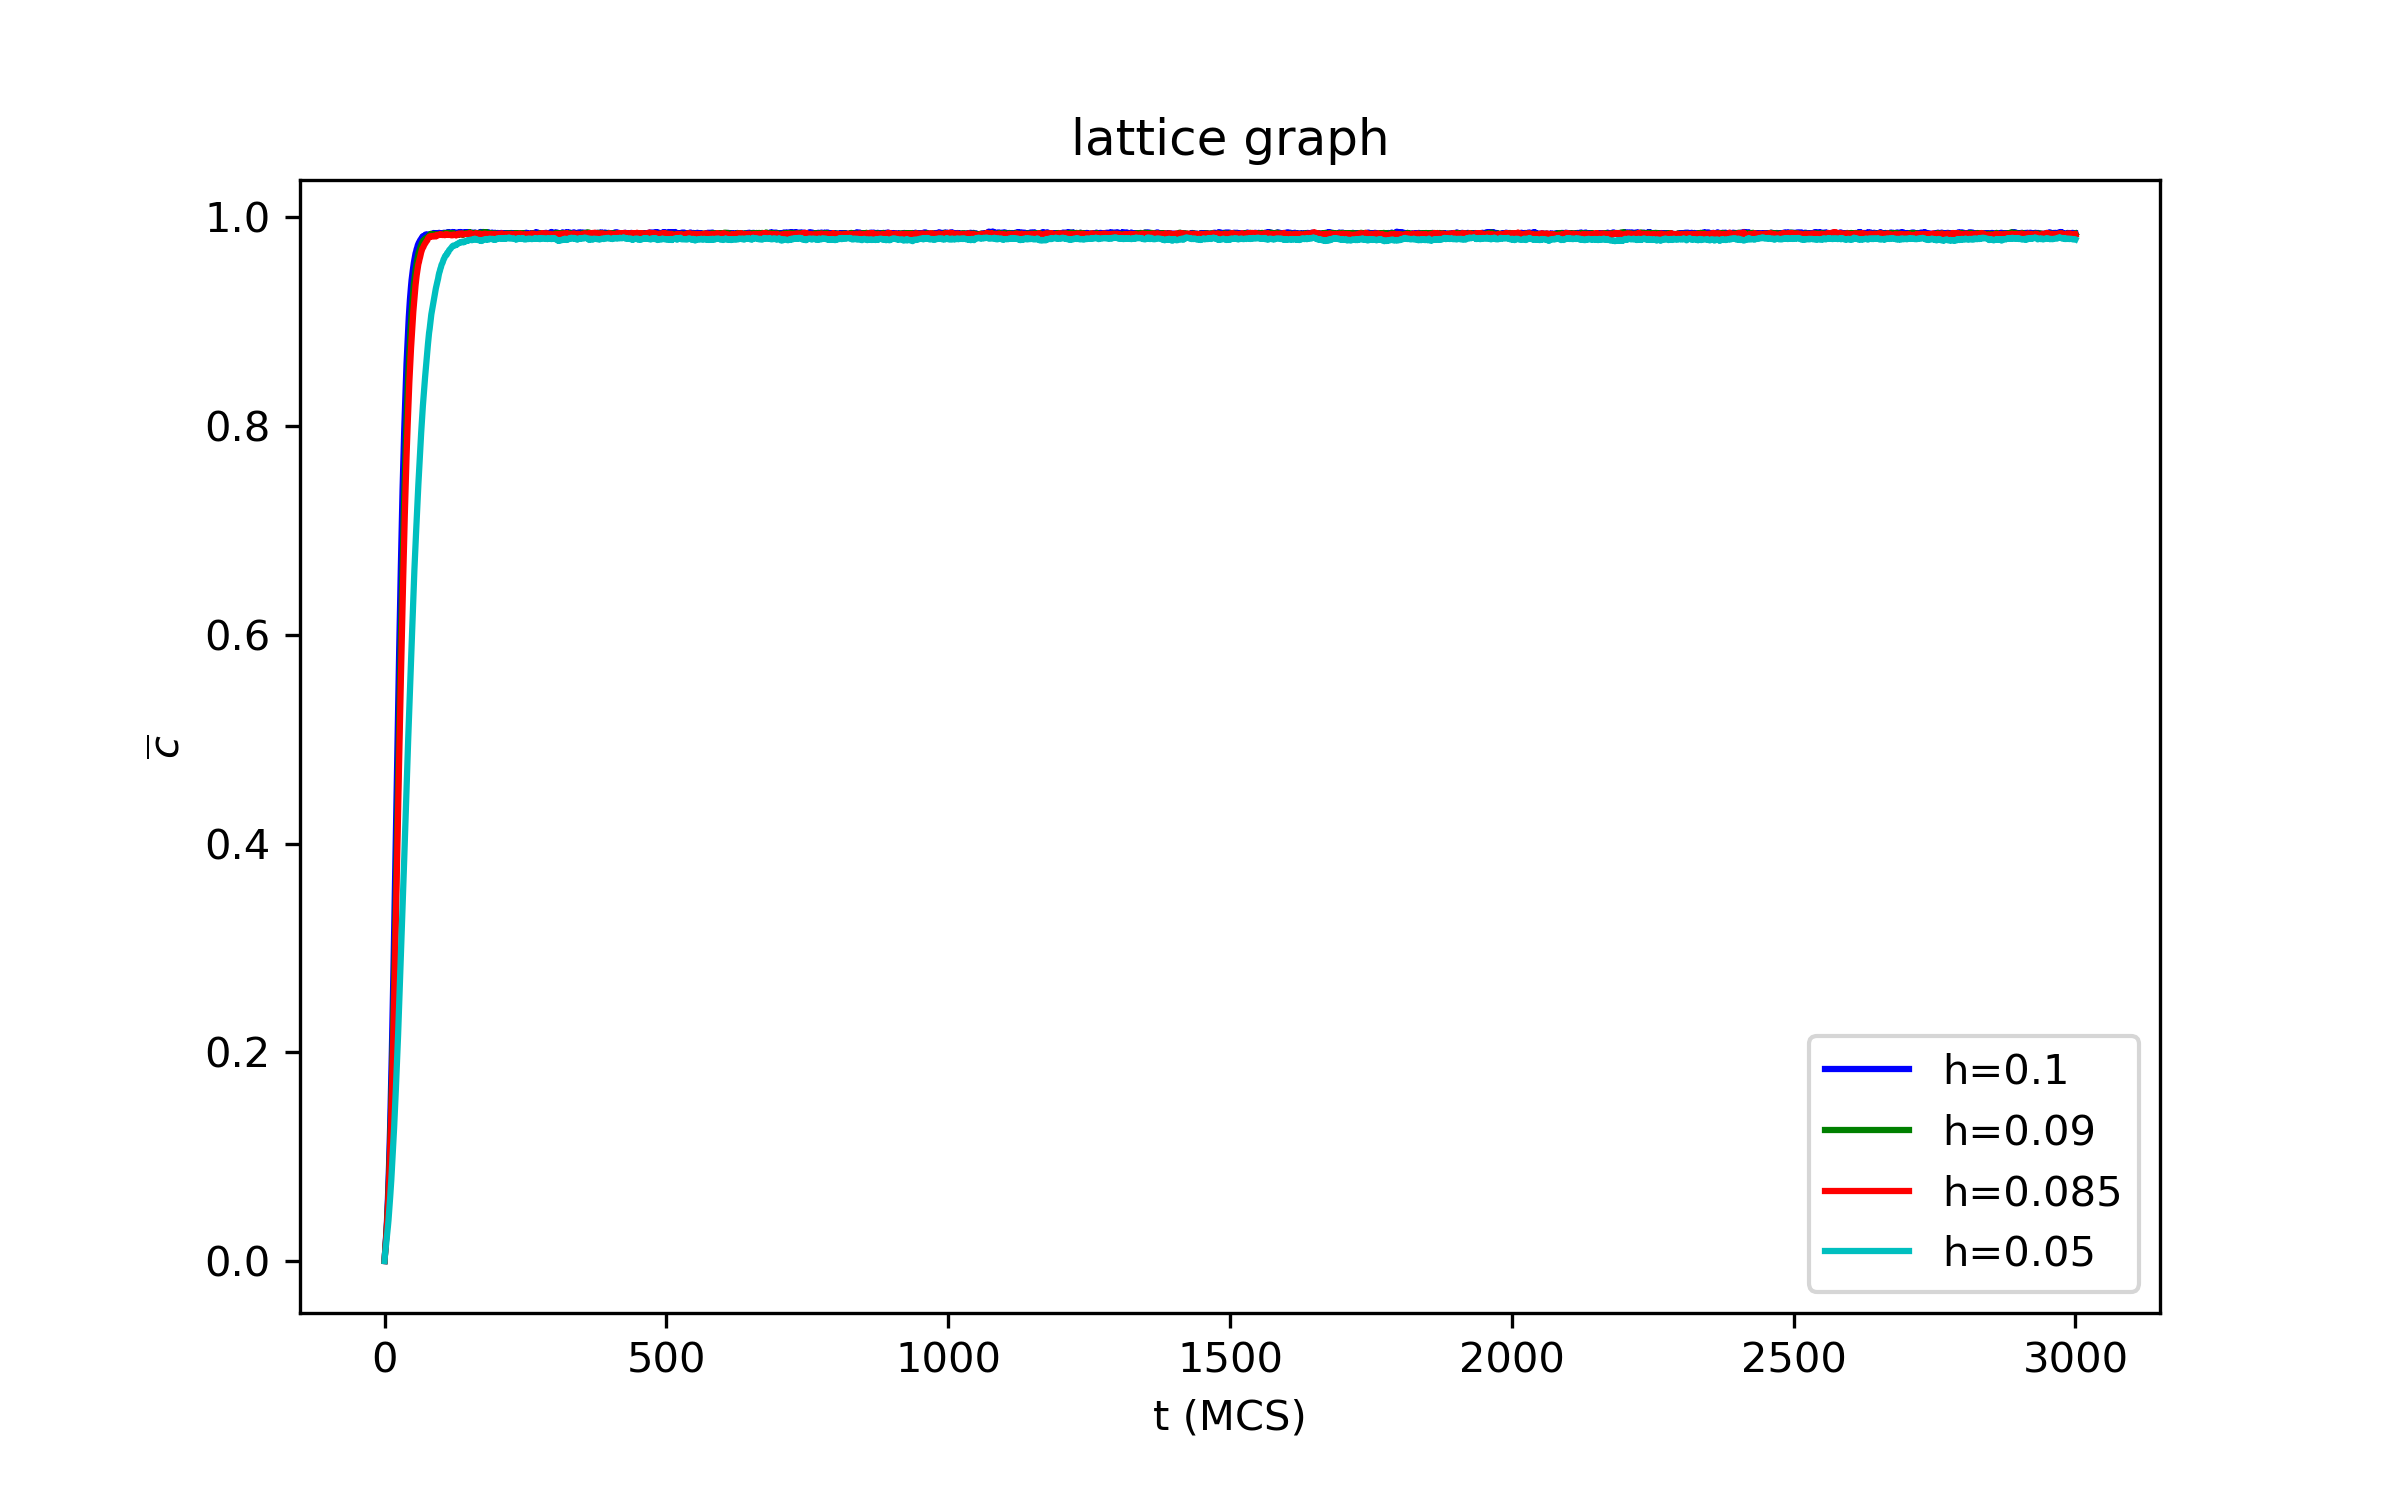
\includegraphics[width=5.5cm, height=4cm]{../results/images/lattice_900.png}
		\caption{Left - publication; right - our simulation with 3000 MC steps and 100 independent runs on a grid lattice with 900 nodes. .}
	\end{figure}
\end{frame}

\begin{frame}{Complete graph results}
	\begin{figure}
		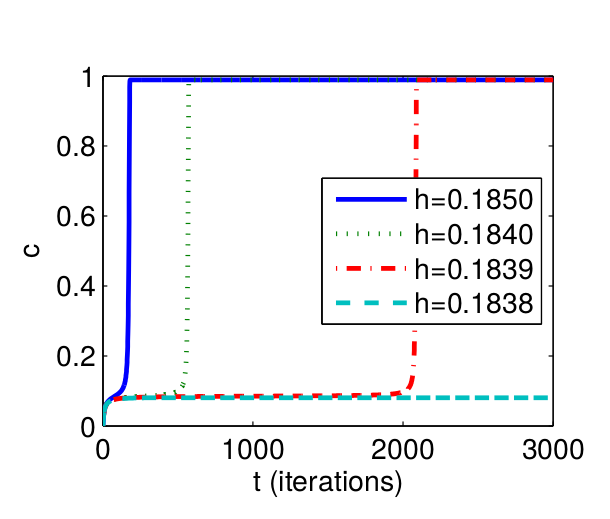
\includegraphics[width=0.475\textwidth]{../resources/images/fig10-left.png}
		\hfill
		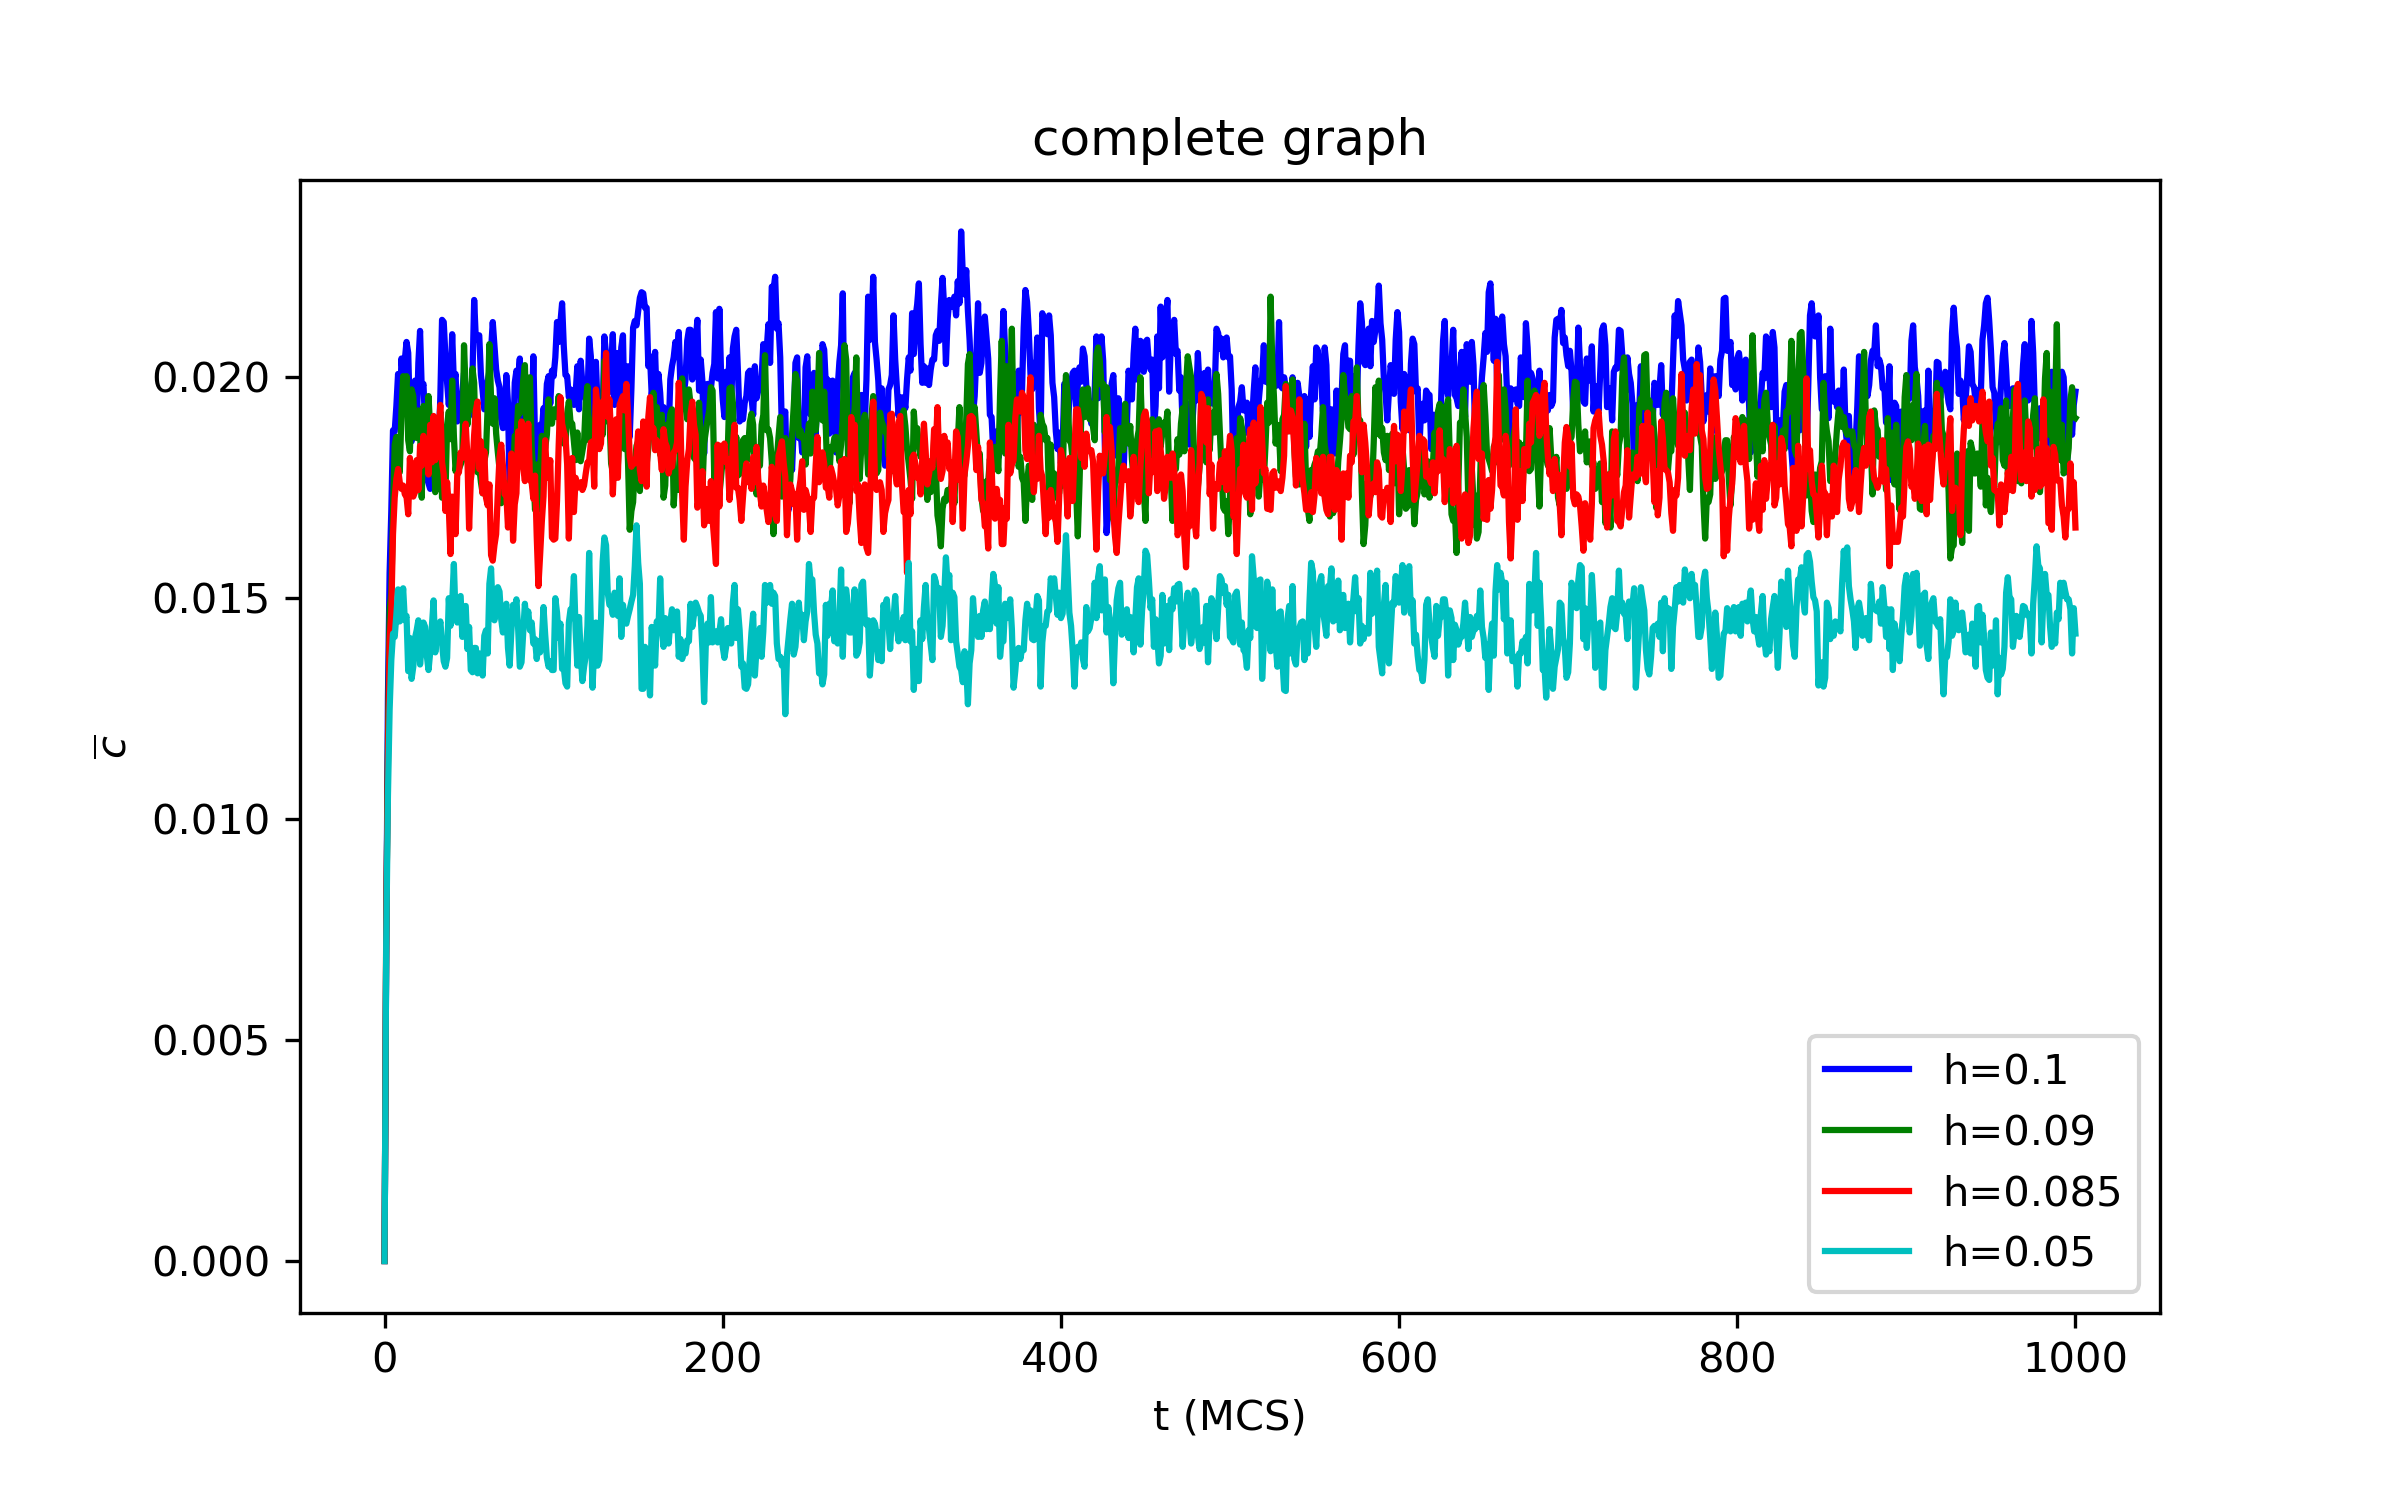
\includegraphics[width=5.5cm, height=4.3cm]{../results/images/complete.png}
		\caption{Left - publication; right - our simulation with 1000 MC steps and 100 independent runs on a complete graph with 400 nodes.  }
	\end{figure}
\end{frame}

\begin{frame}{Watts-Strogatz results}
	\begin{figure}
		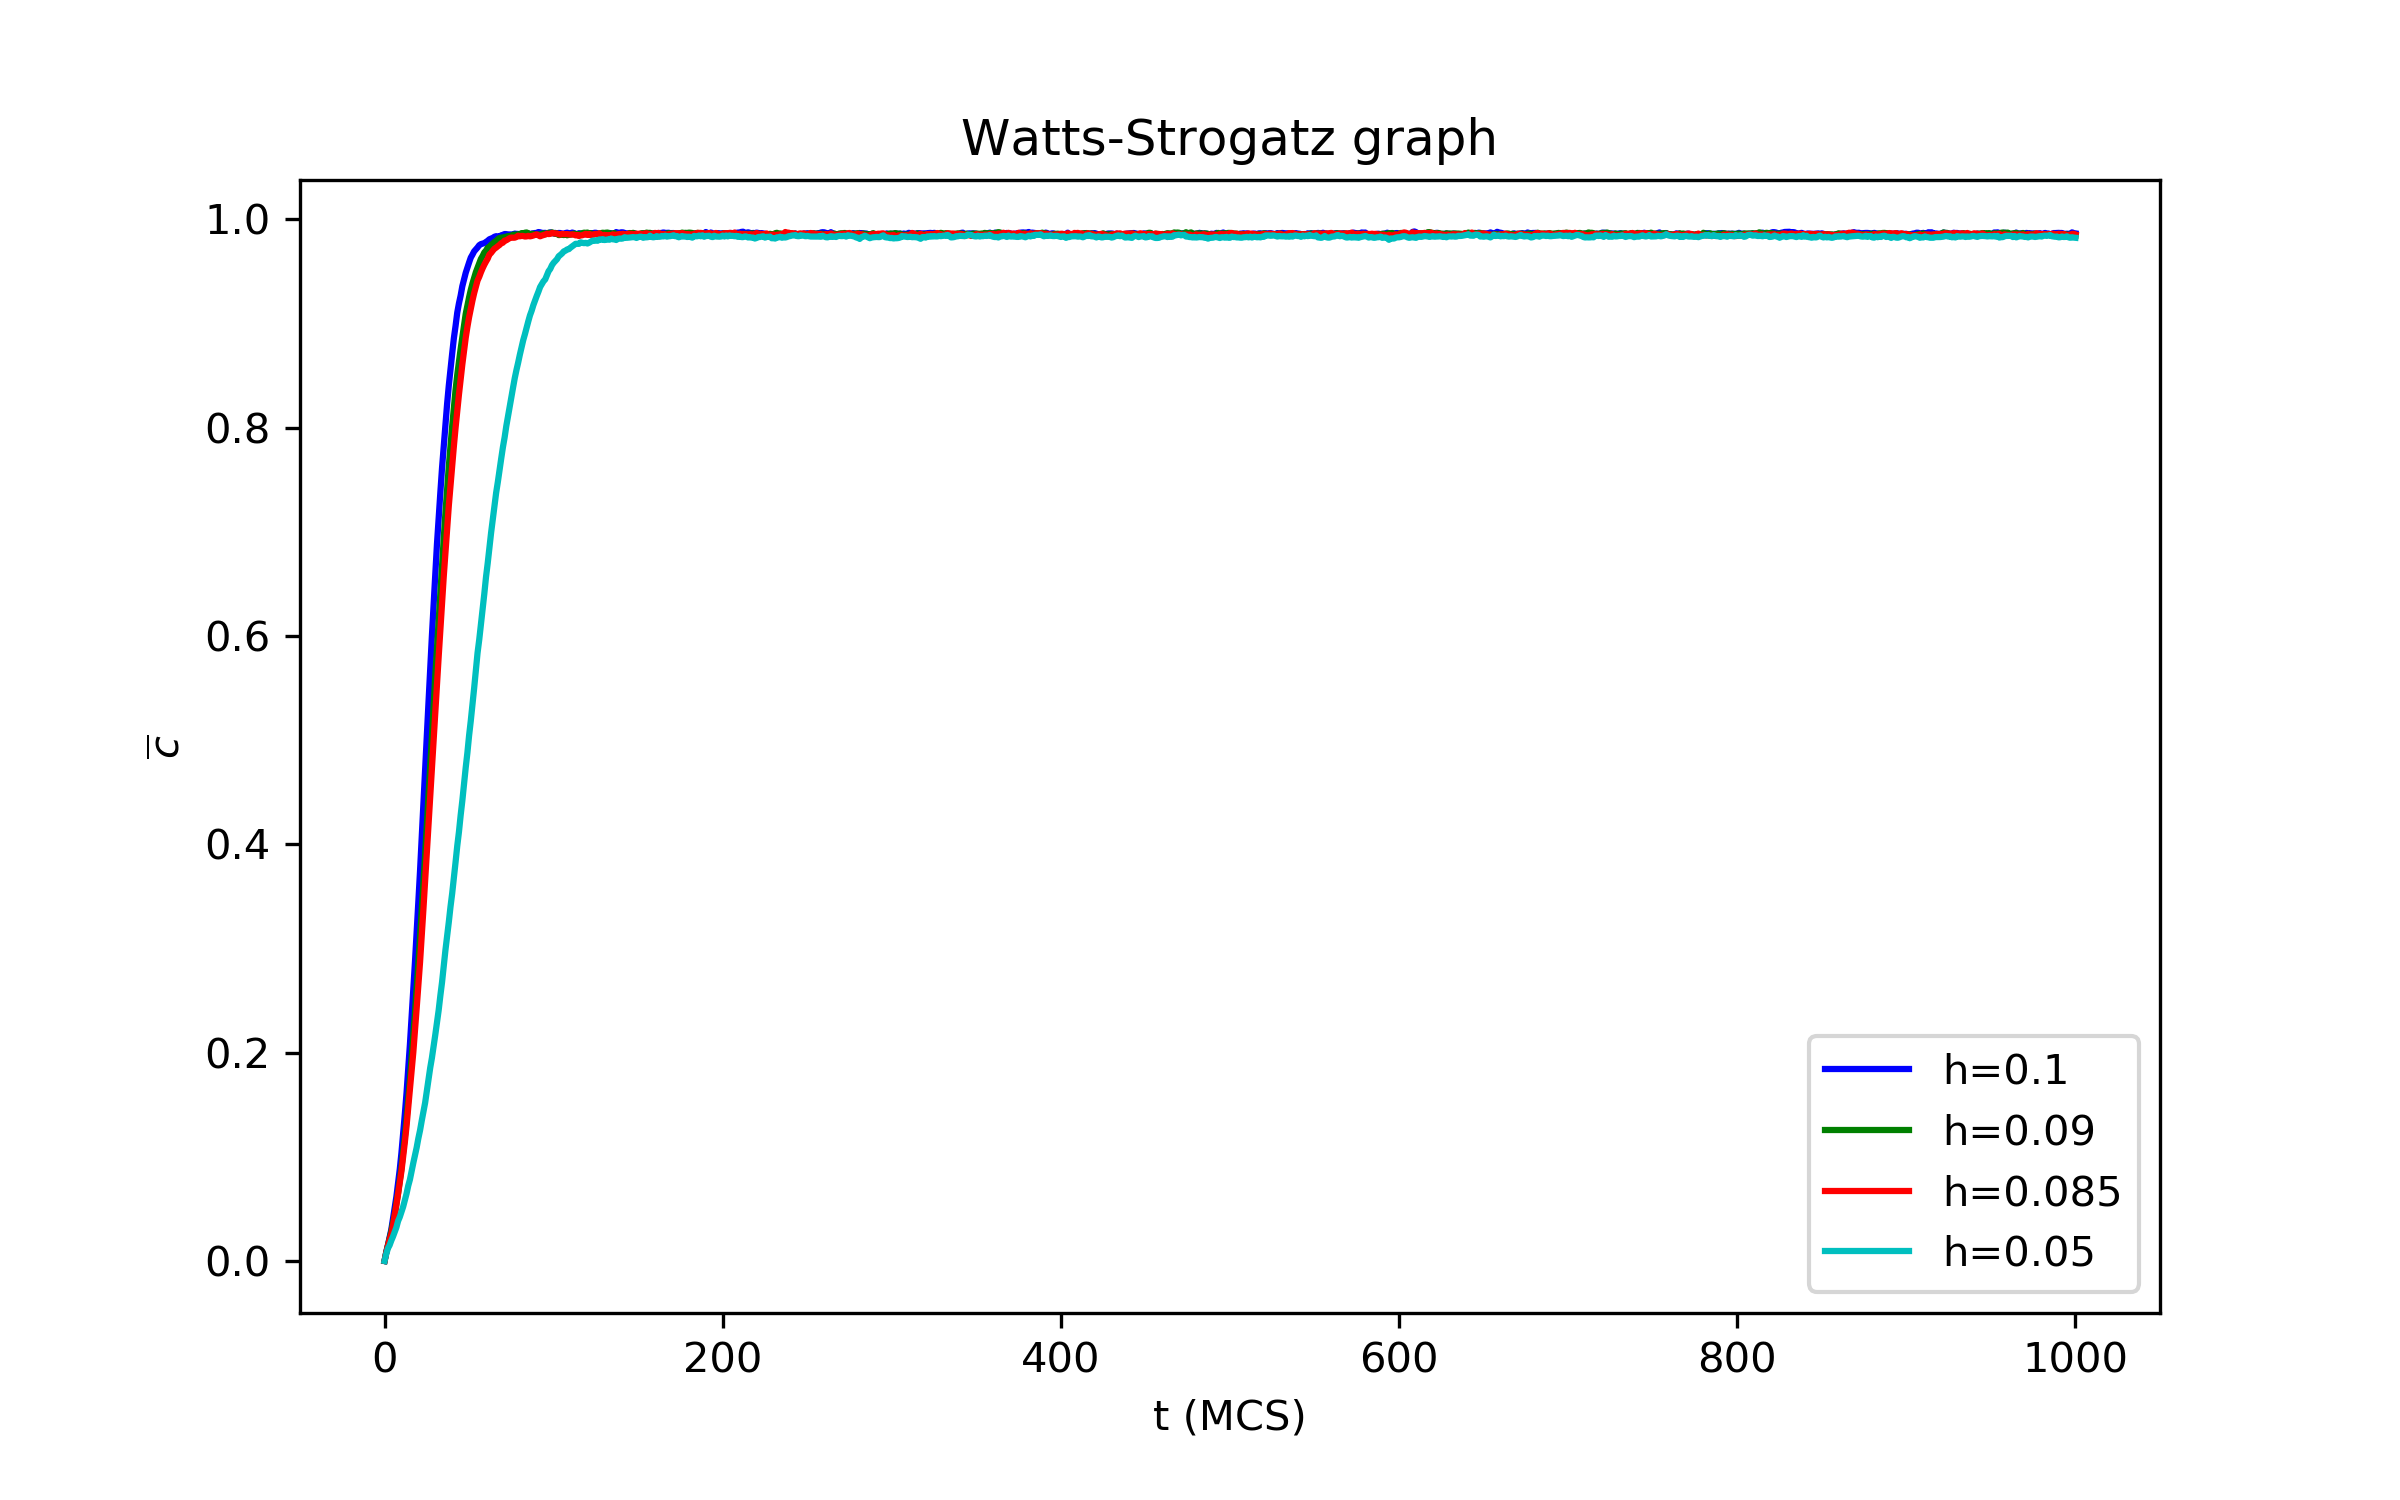
\includegraphics[width=\textwidth]{../results/images/WS.png}
		\caption{Our work - simulation with 1000 MC steps and 100 independent runs on a Watts-Strogatz (k=4,p=0.3) graph with 400 nodes. }
	\end{figure}
\end{frame}

\begin{frame}{Barabasi-Albert results}
	\begin{figure}
		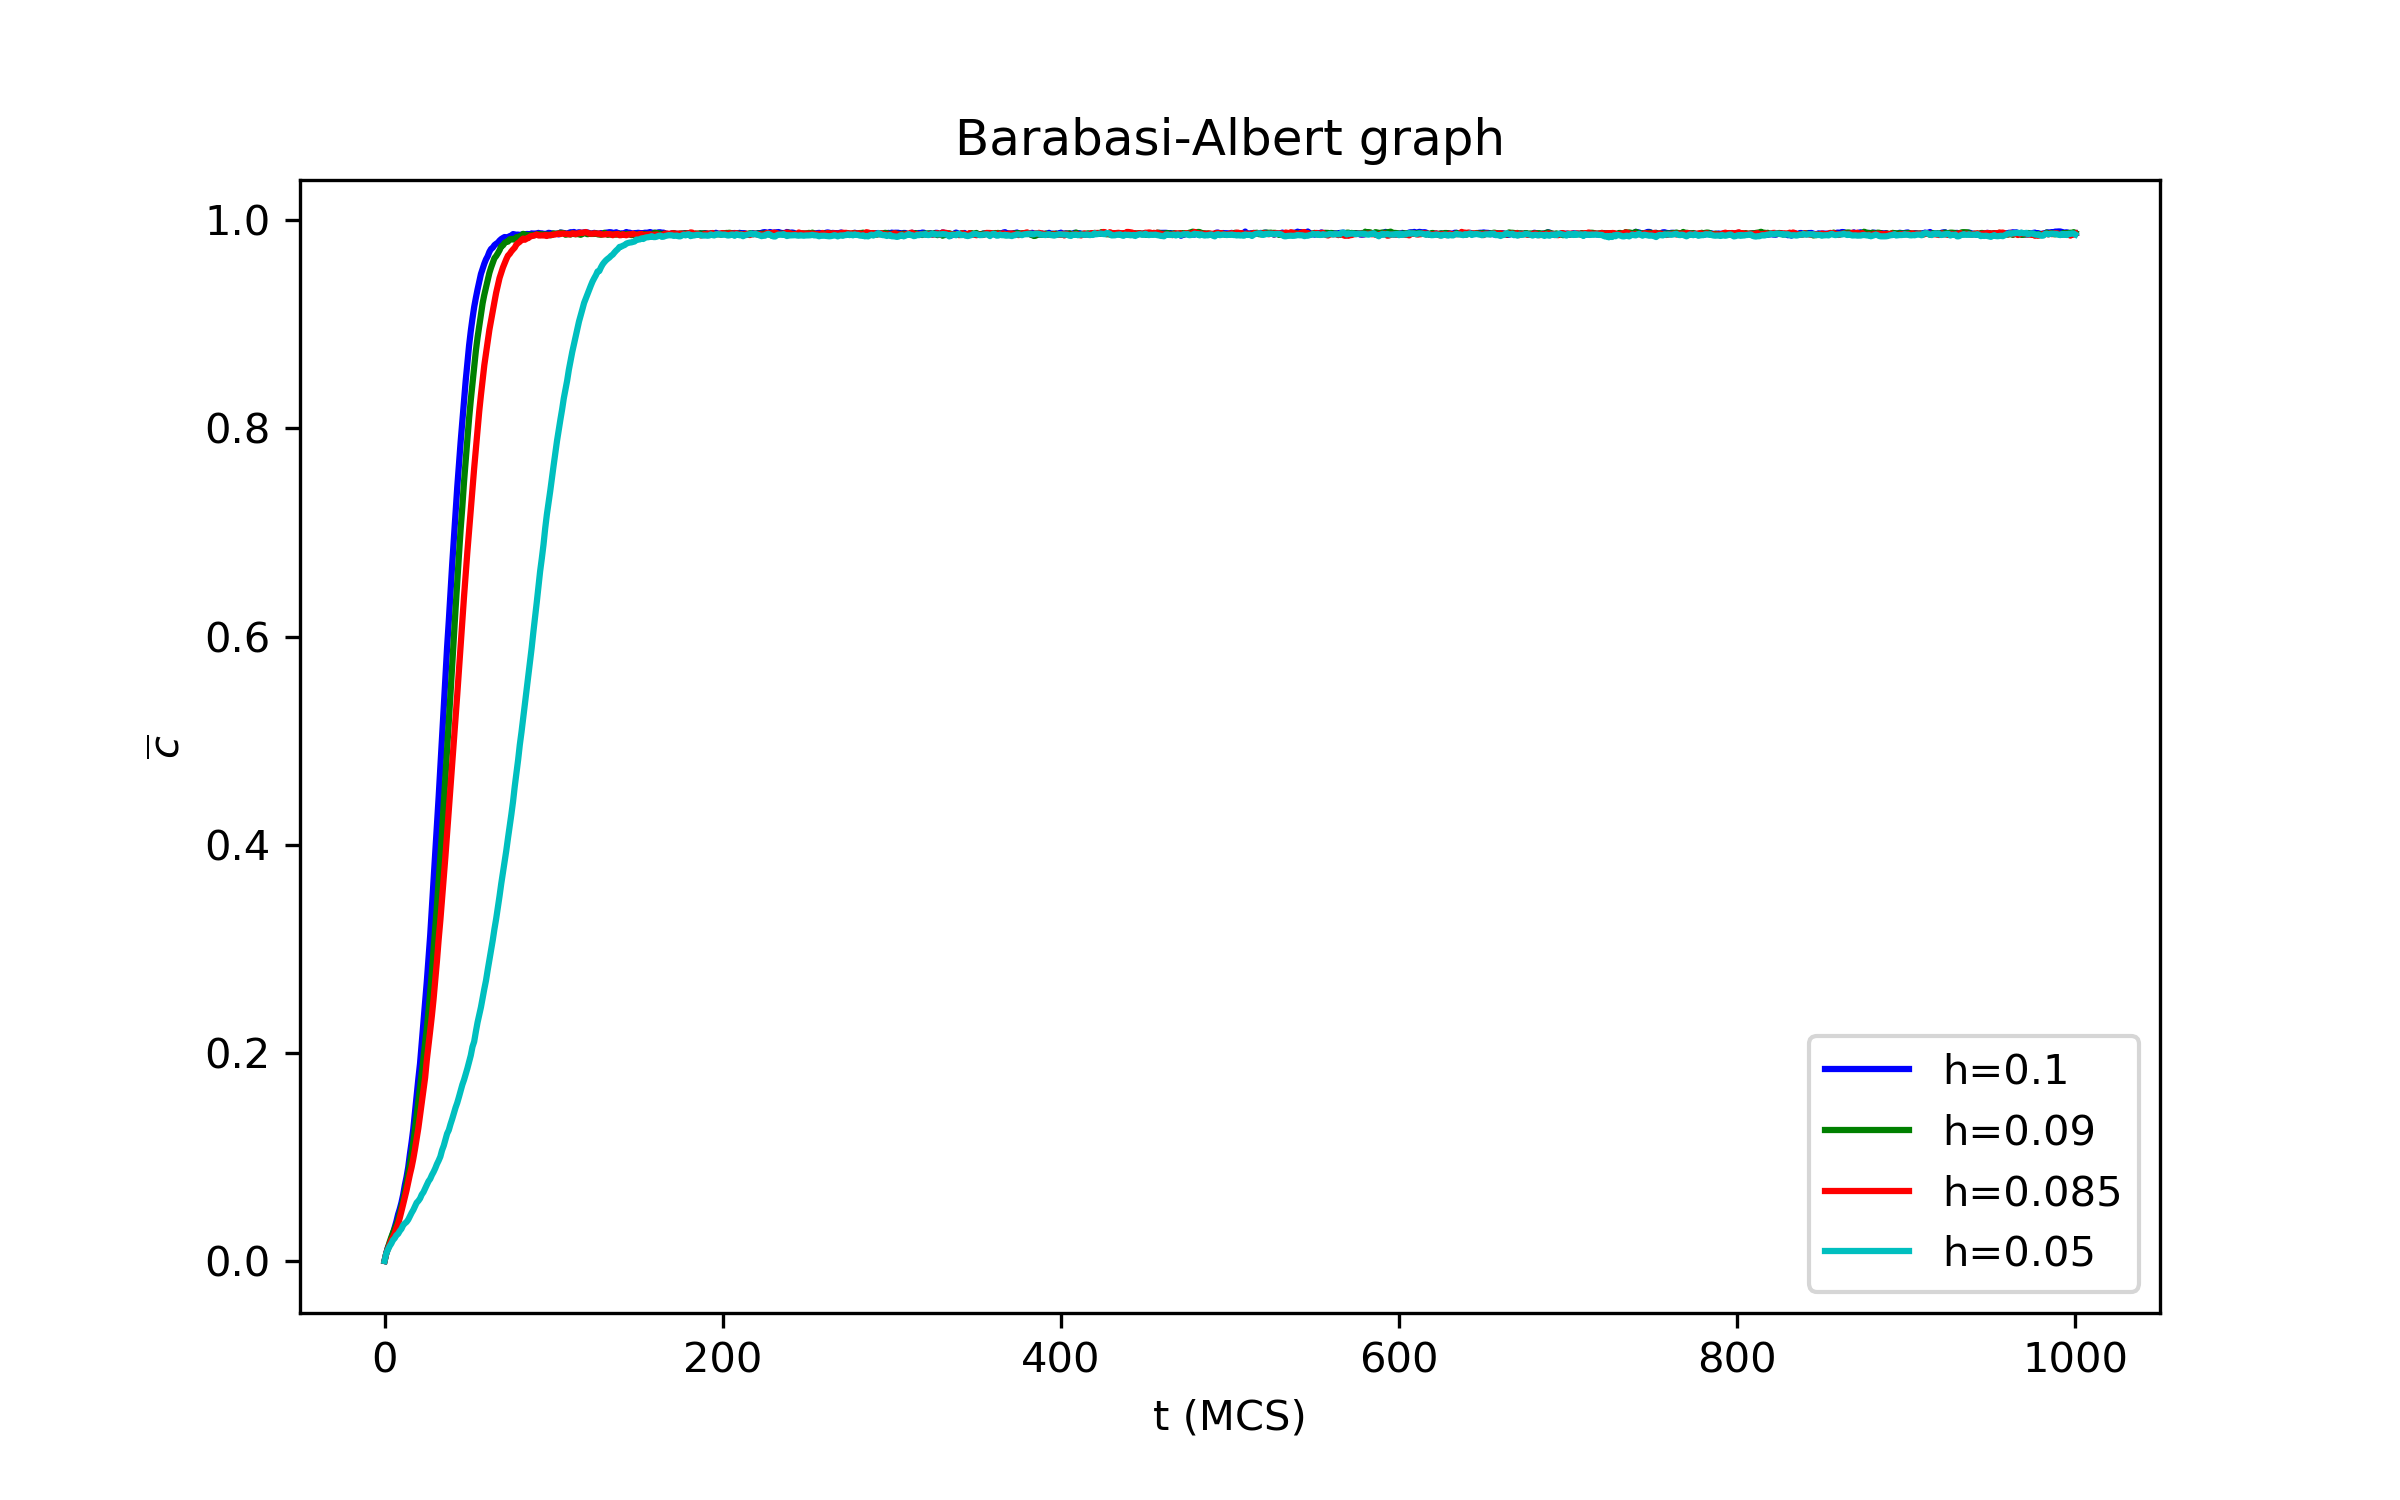
\includegraphics[width=\textwidth]{../results/images/BA.png}
		\caption{Our work - simulation with 1000 MC steps and 100 independent runs on a Barabasi-Albert (2) graph with 400 nodes. }
	\end{figure}
\end{frame}

\begin{frame}{Comparison of models}
	\begin{figure}
		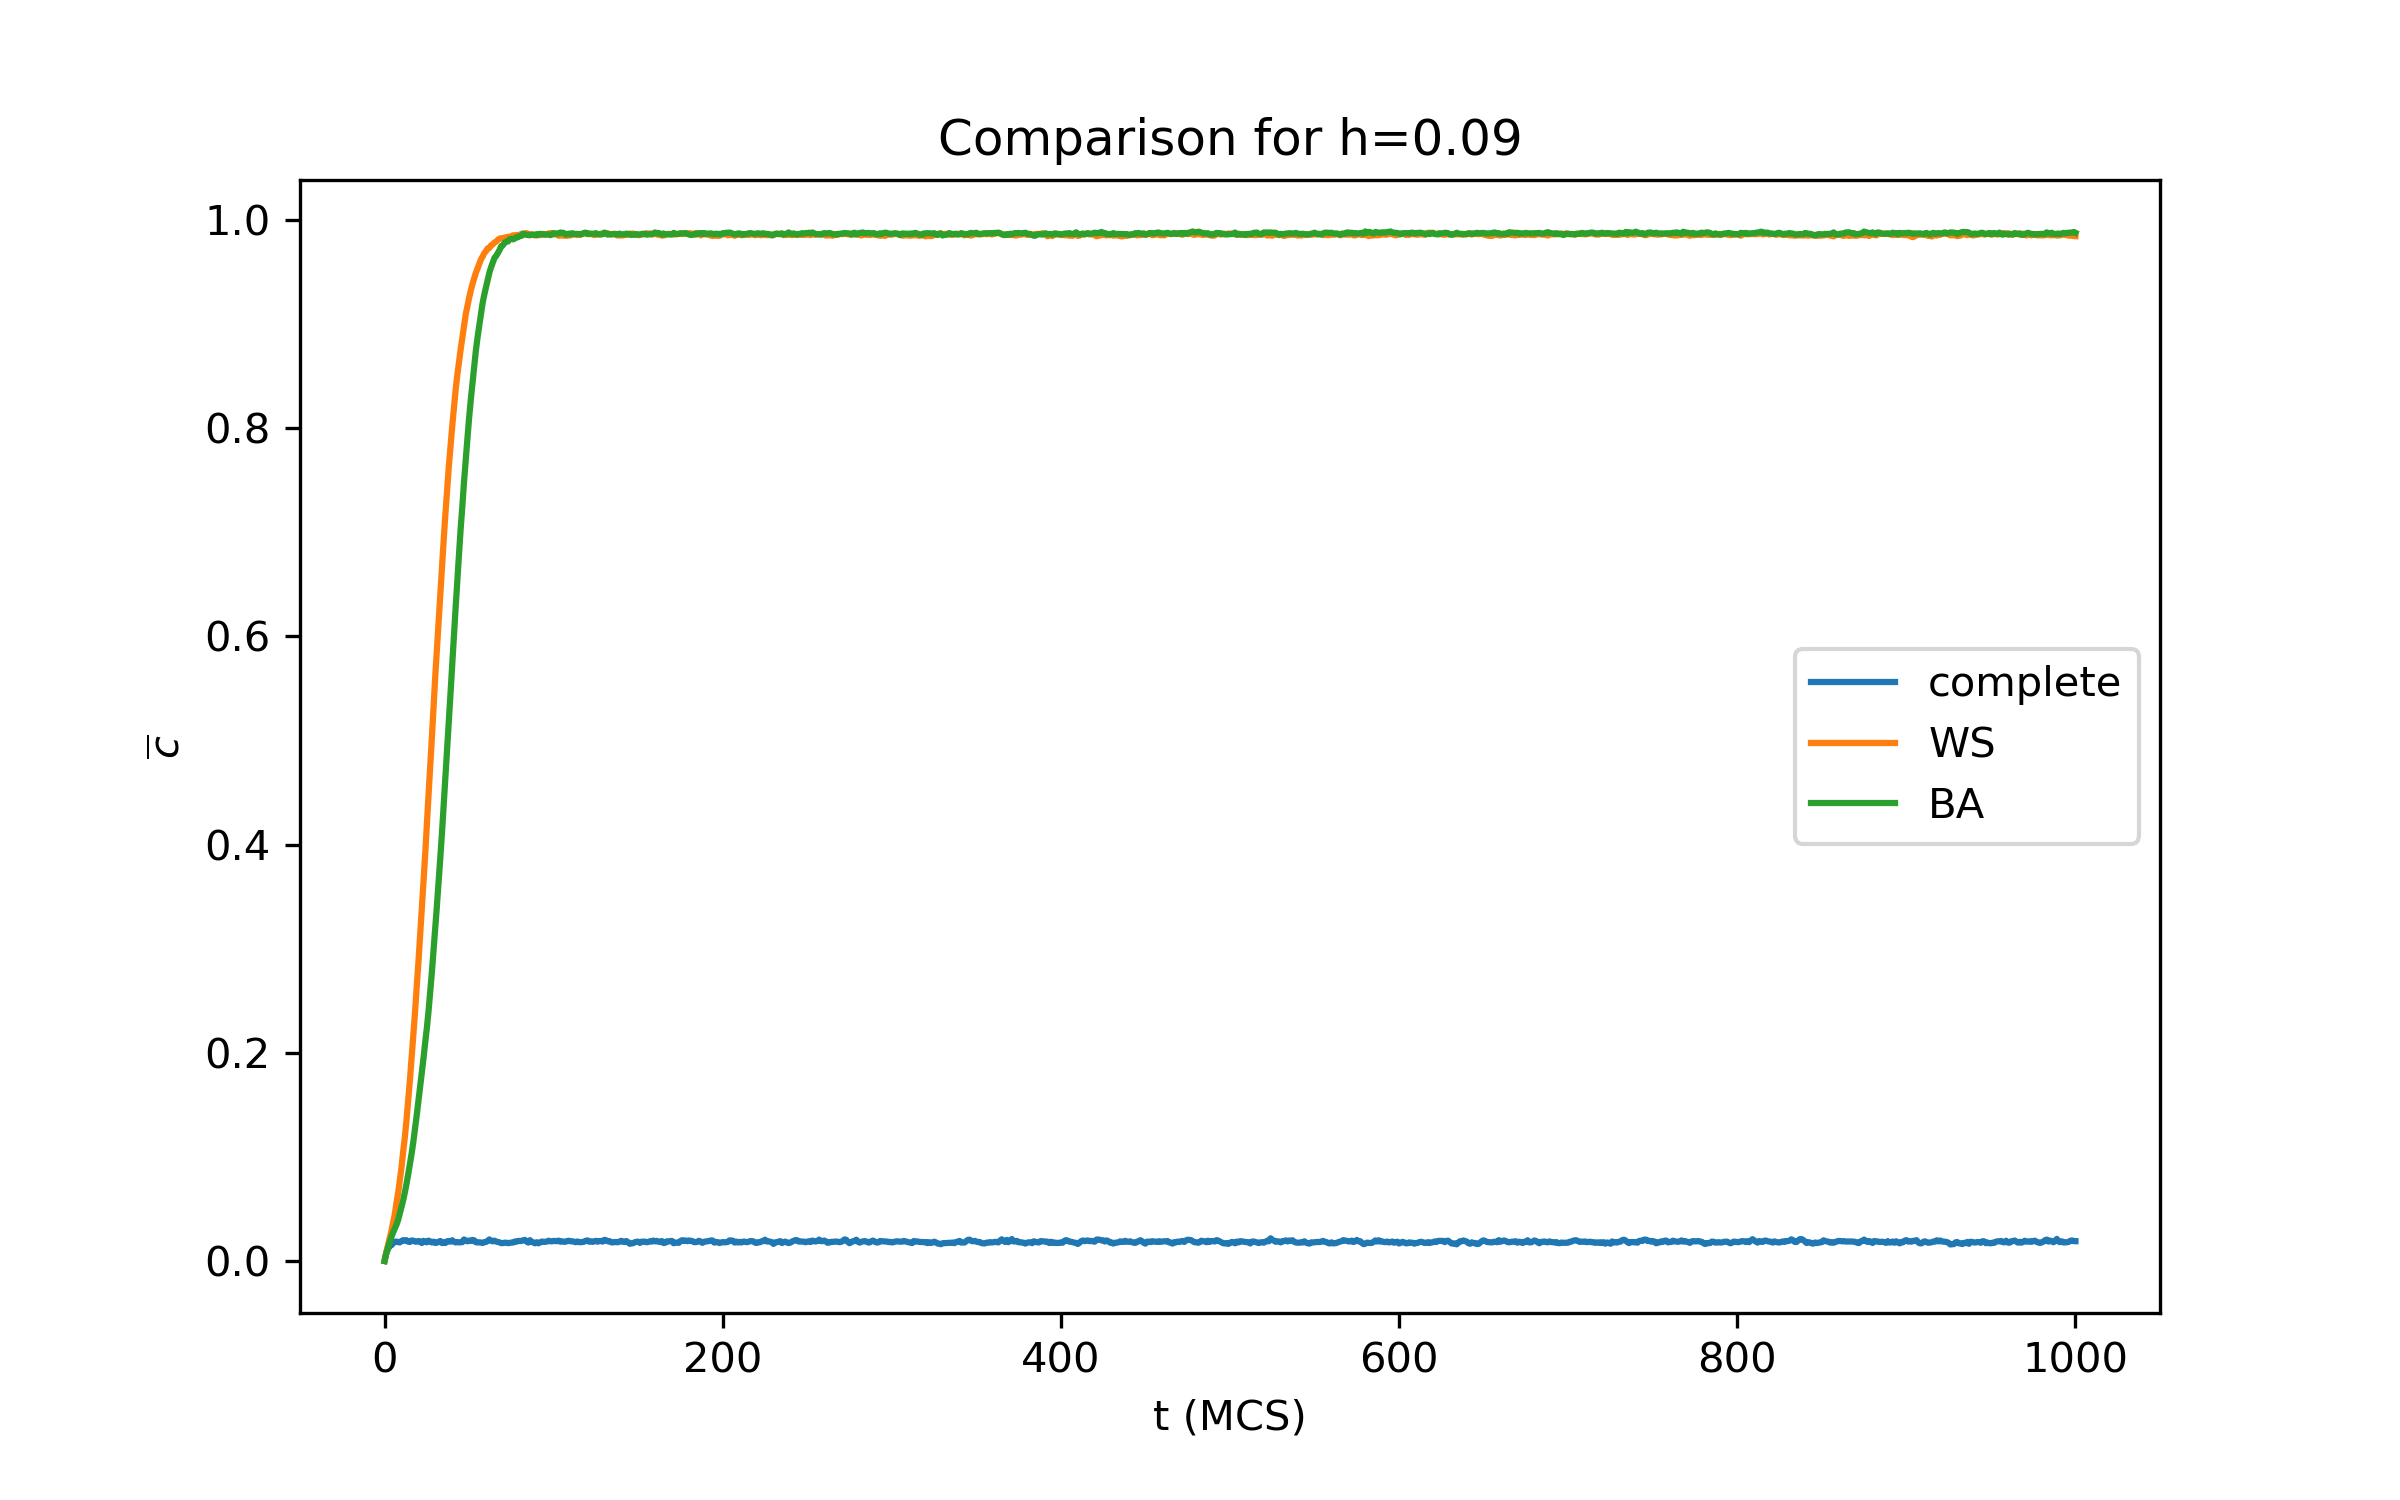
\includegraphics[width=\textwidth]{../results/images/comparison.png}
		\caption{Our work - simulation with 1000 MC steps and 100 independent runs on graphs with 400 nodes, h=0.09. }
	\end{figure}
\end{frame}

\section{Market penetration level}

\begin{frame}{Valley of death}
	Valley of death is a metaphor of way from the laboratory to the market when in reality many innovators fail. Contrary to aggregate models, such as Bass model, this kind of phenomena can be explained by agent-based models.
	
	We can observe that phenomenon near the threshold values of $p$ and $h$.
\end{frame}

\begin{frame}{2D Lattice results}
	\begin{figure}
		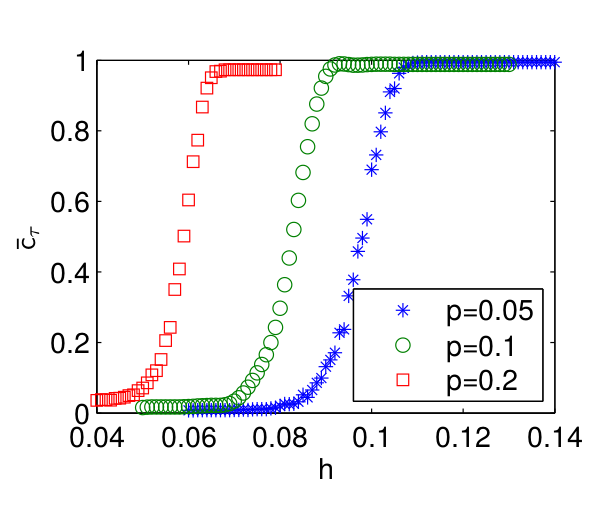
\includegraphics[width=0.475\textwidth]{../resources/images/fig9-left.png}
		\hfill
		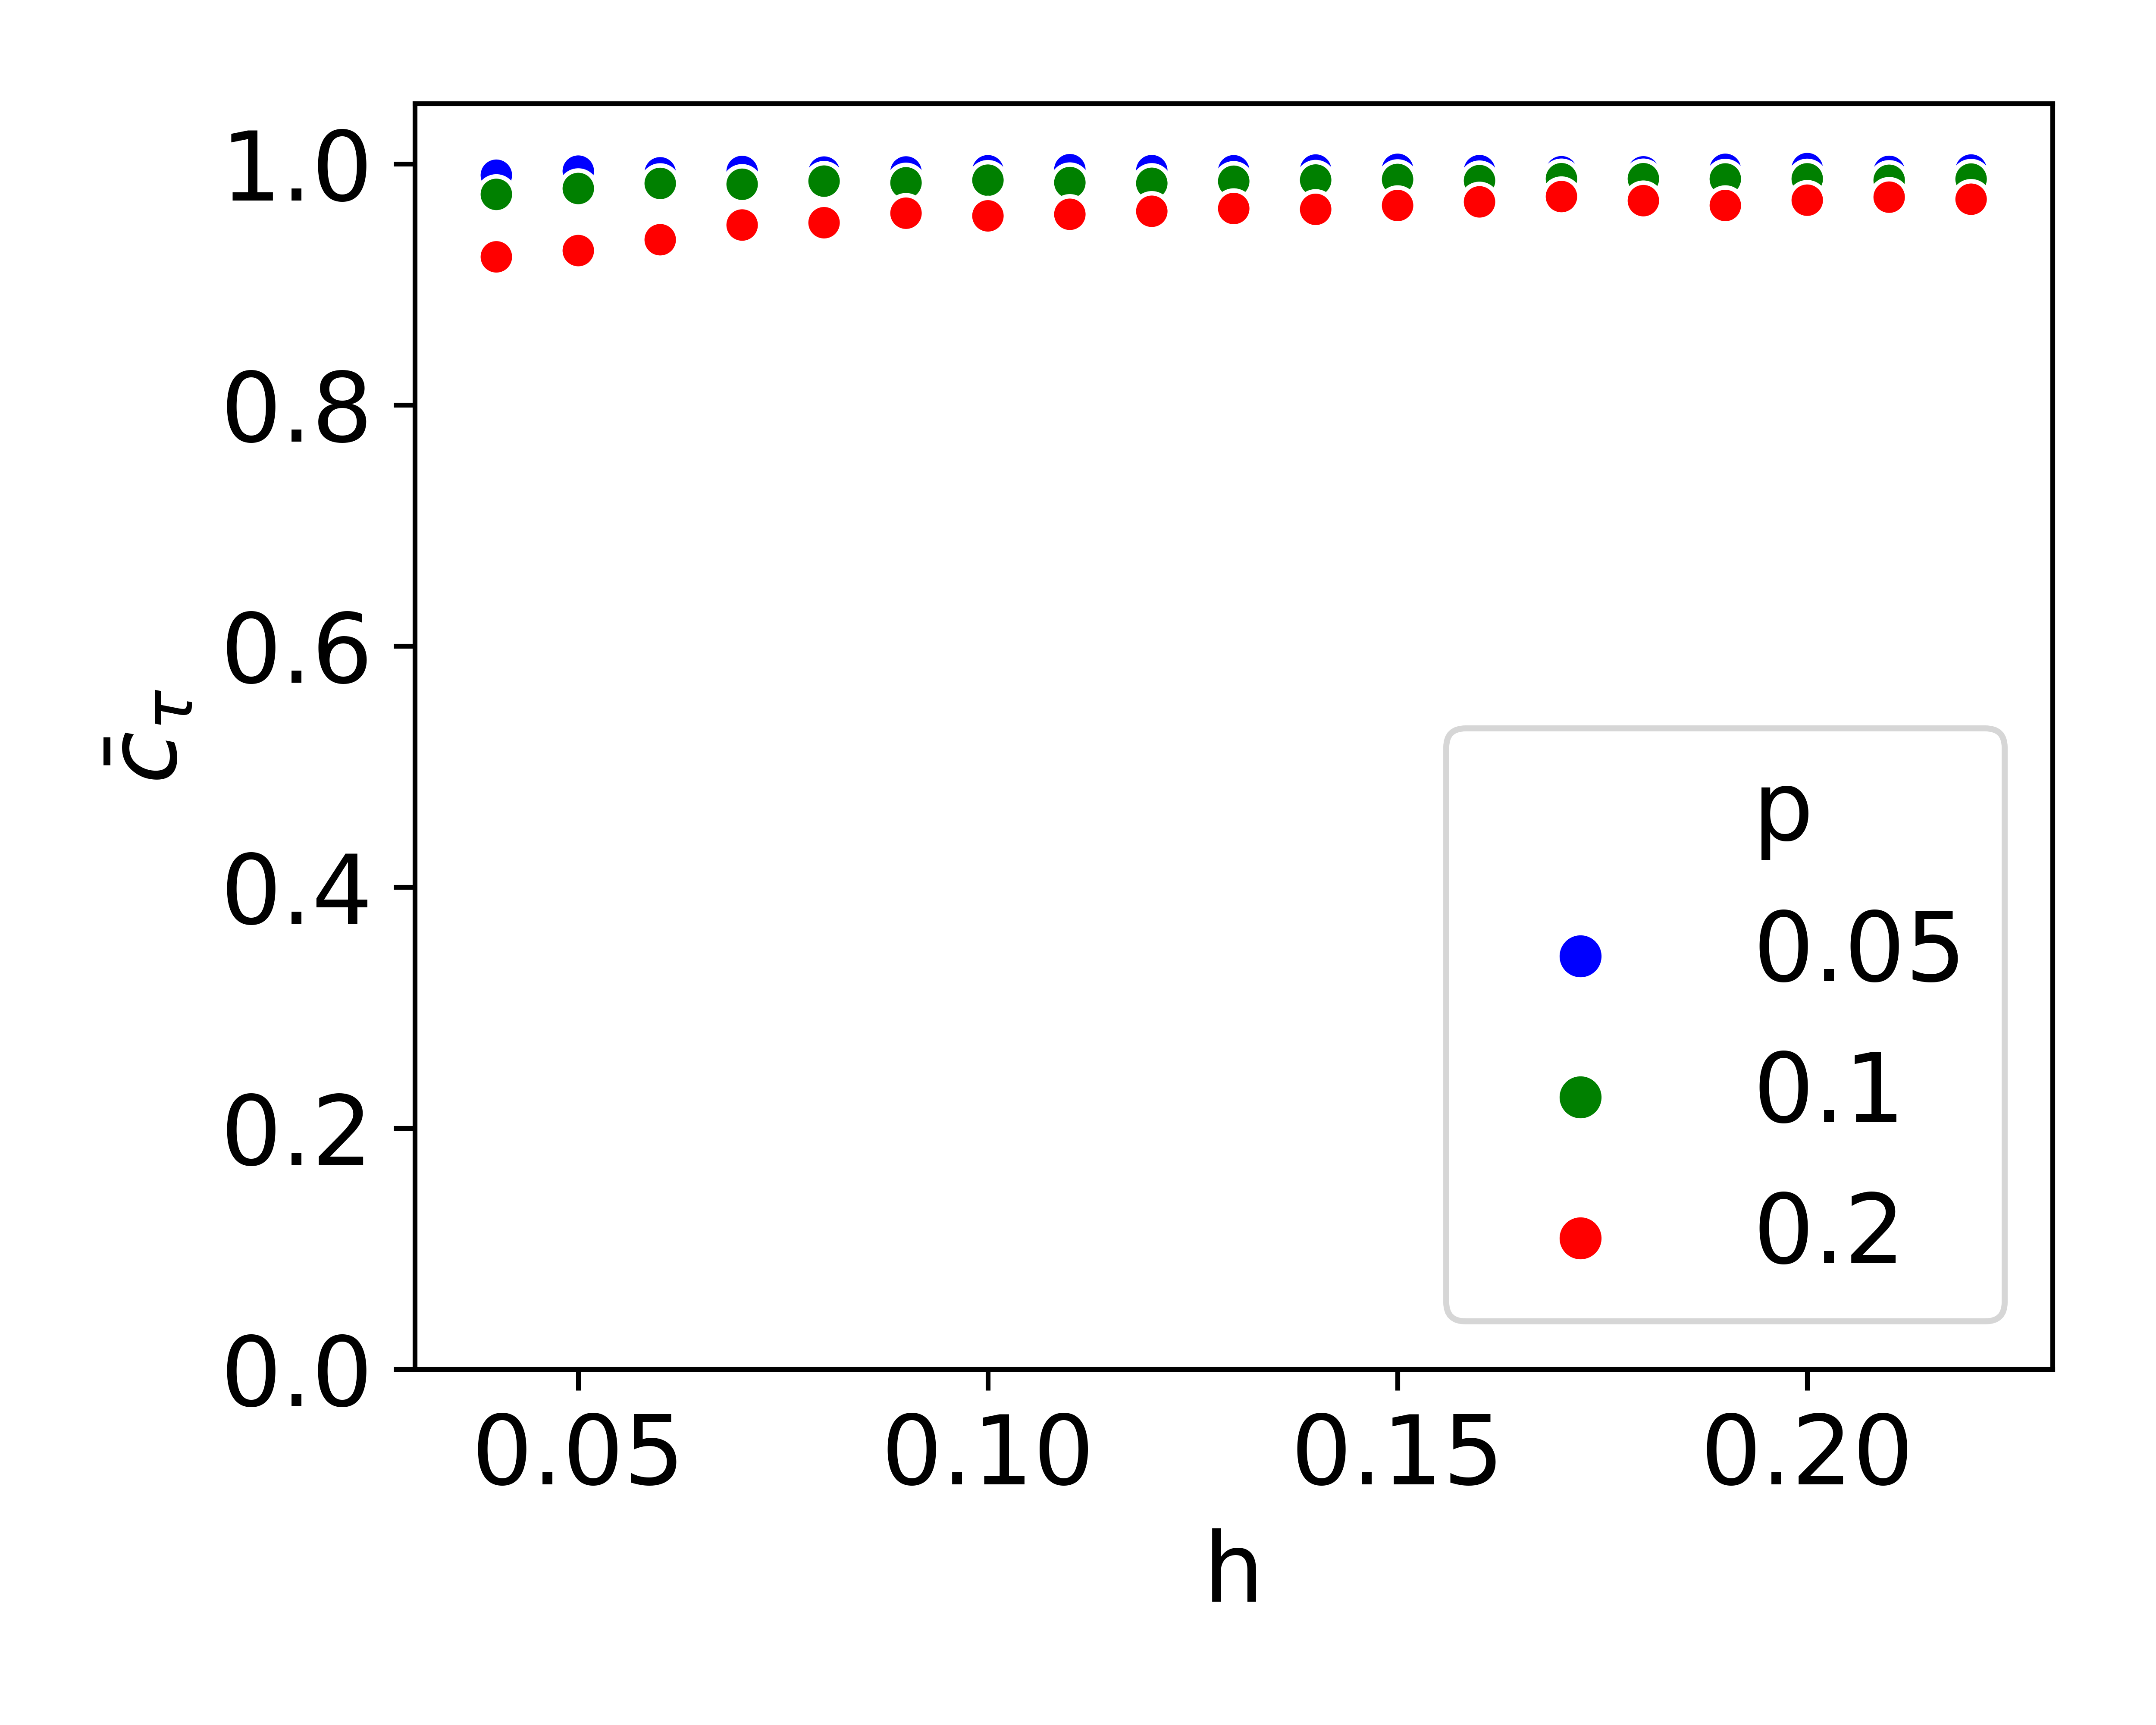
\includegraphics[width=0.475\textwidth]{../results/images/hp-lattice.png}
		\caption{Left - publication; right - ours.}
	\end{figure}
	Comparison - Fig. 9 (left)
	Simulations
\end{frame}

\begin{frame}{Complete graph results}
	\begin{figure}
		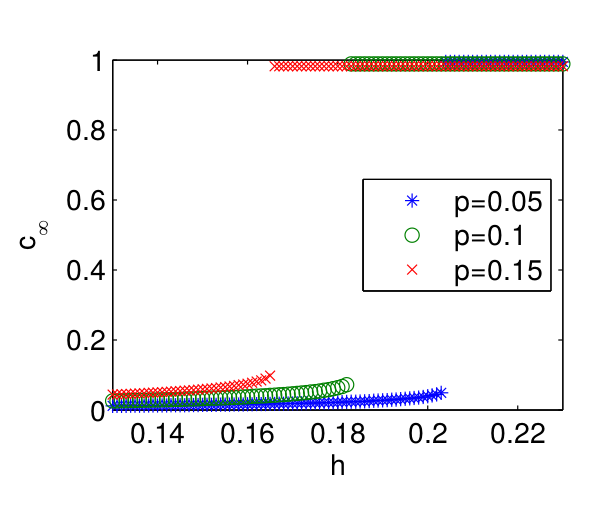
\includegraphics[width=0.475\textwidth]{../resources/images/fig10-right.png}
		\hfill
		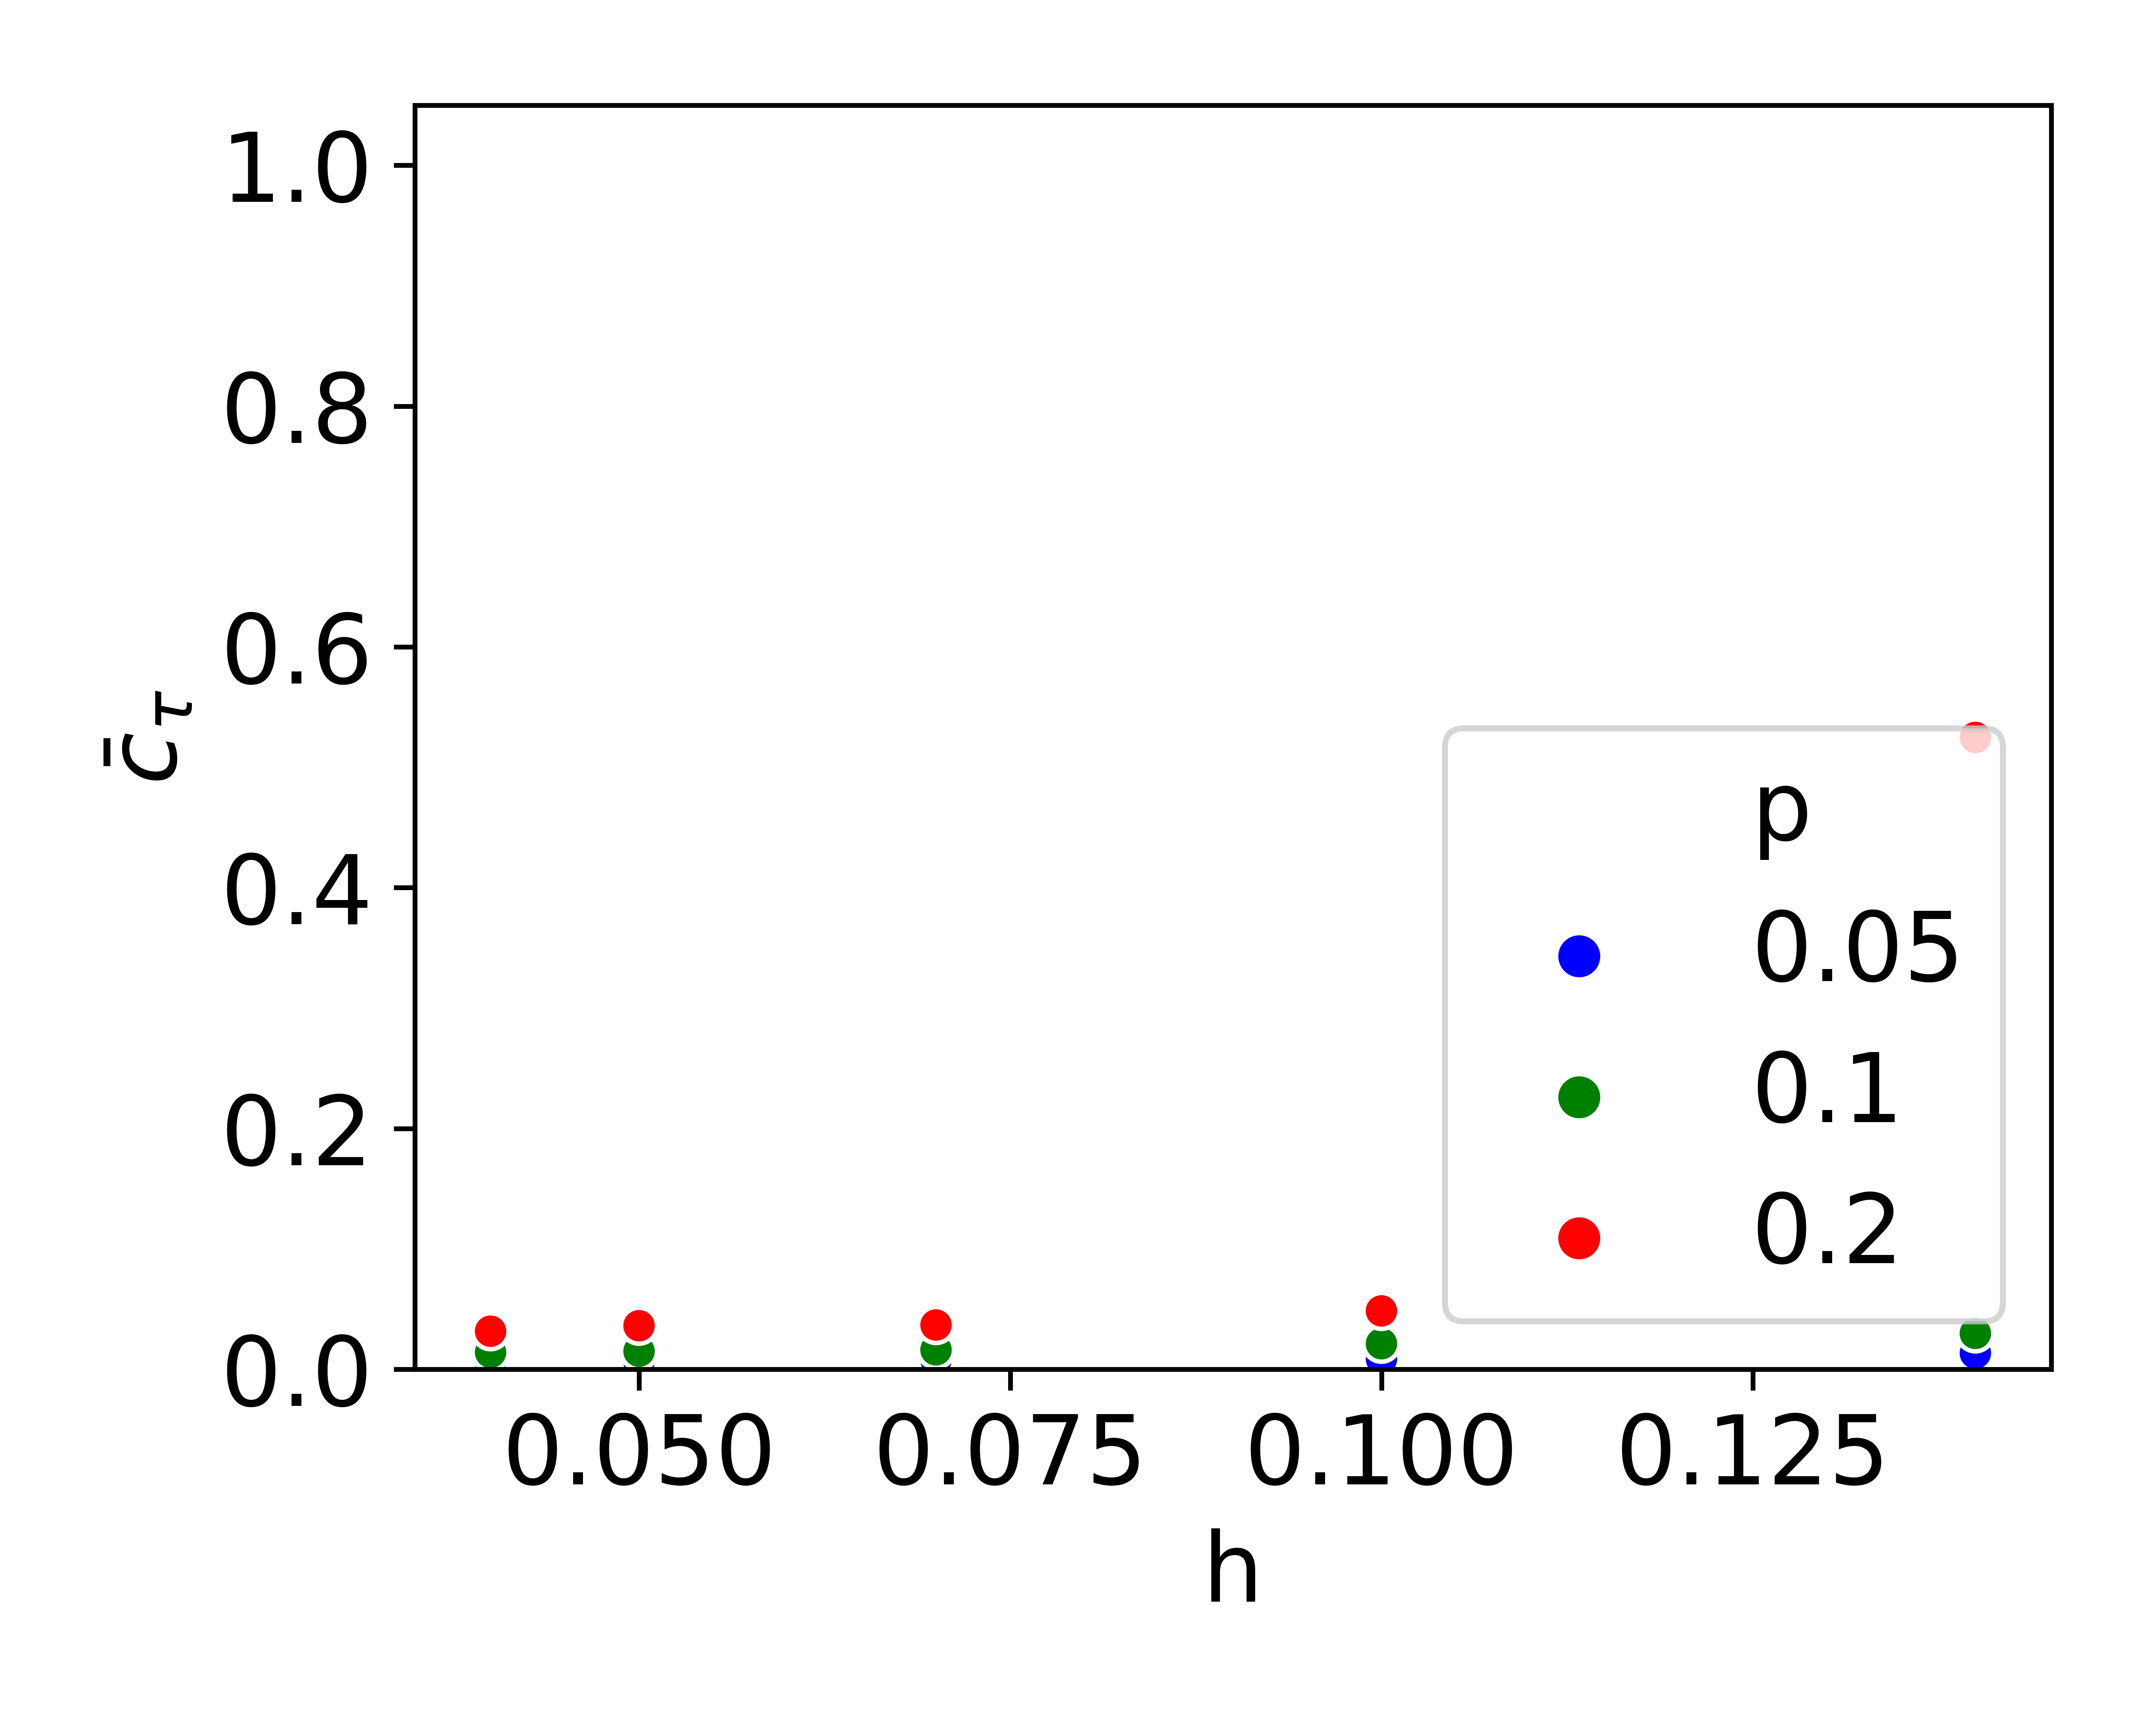
\includegraphics[width=0.475\textwidth]{../results/images/hp-complete.png}
		\caption{Left - publication; right - ours.}
	\end{figure}
	Comparison - Fig. 10 (right)
	Theoretical results
\end{frame}

\begin{frame}{Watts-Strogatz results}
	\begin{figure}
		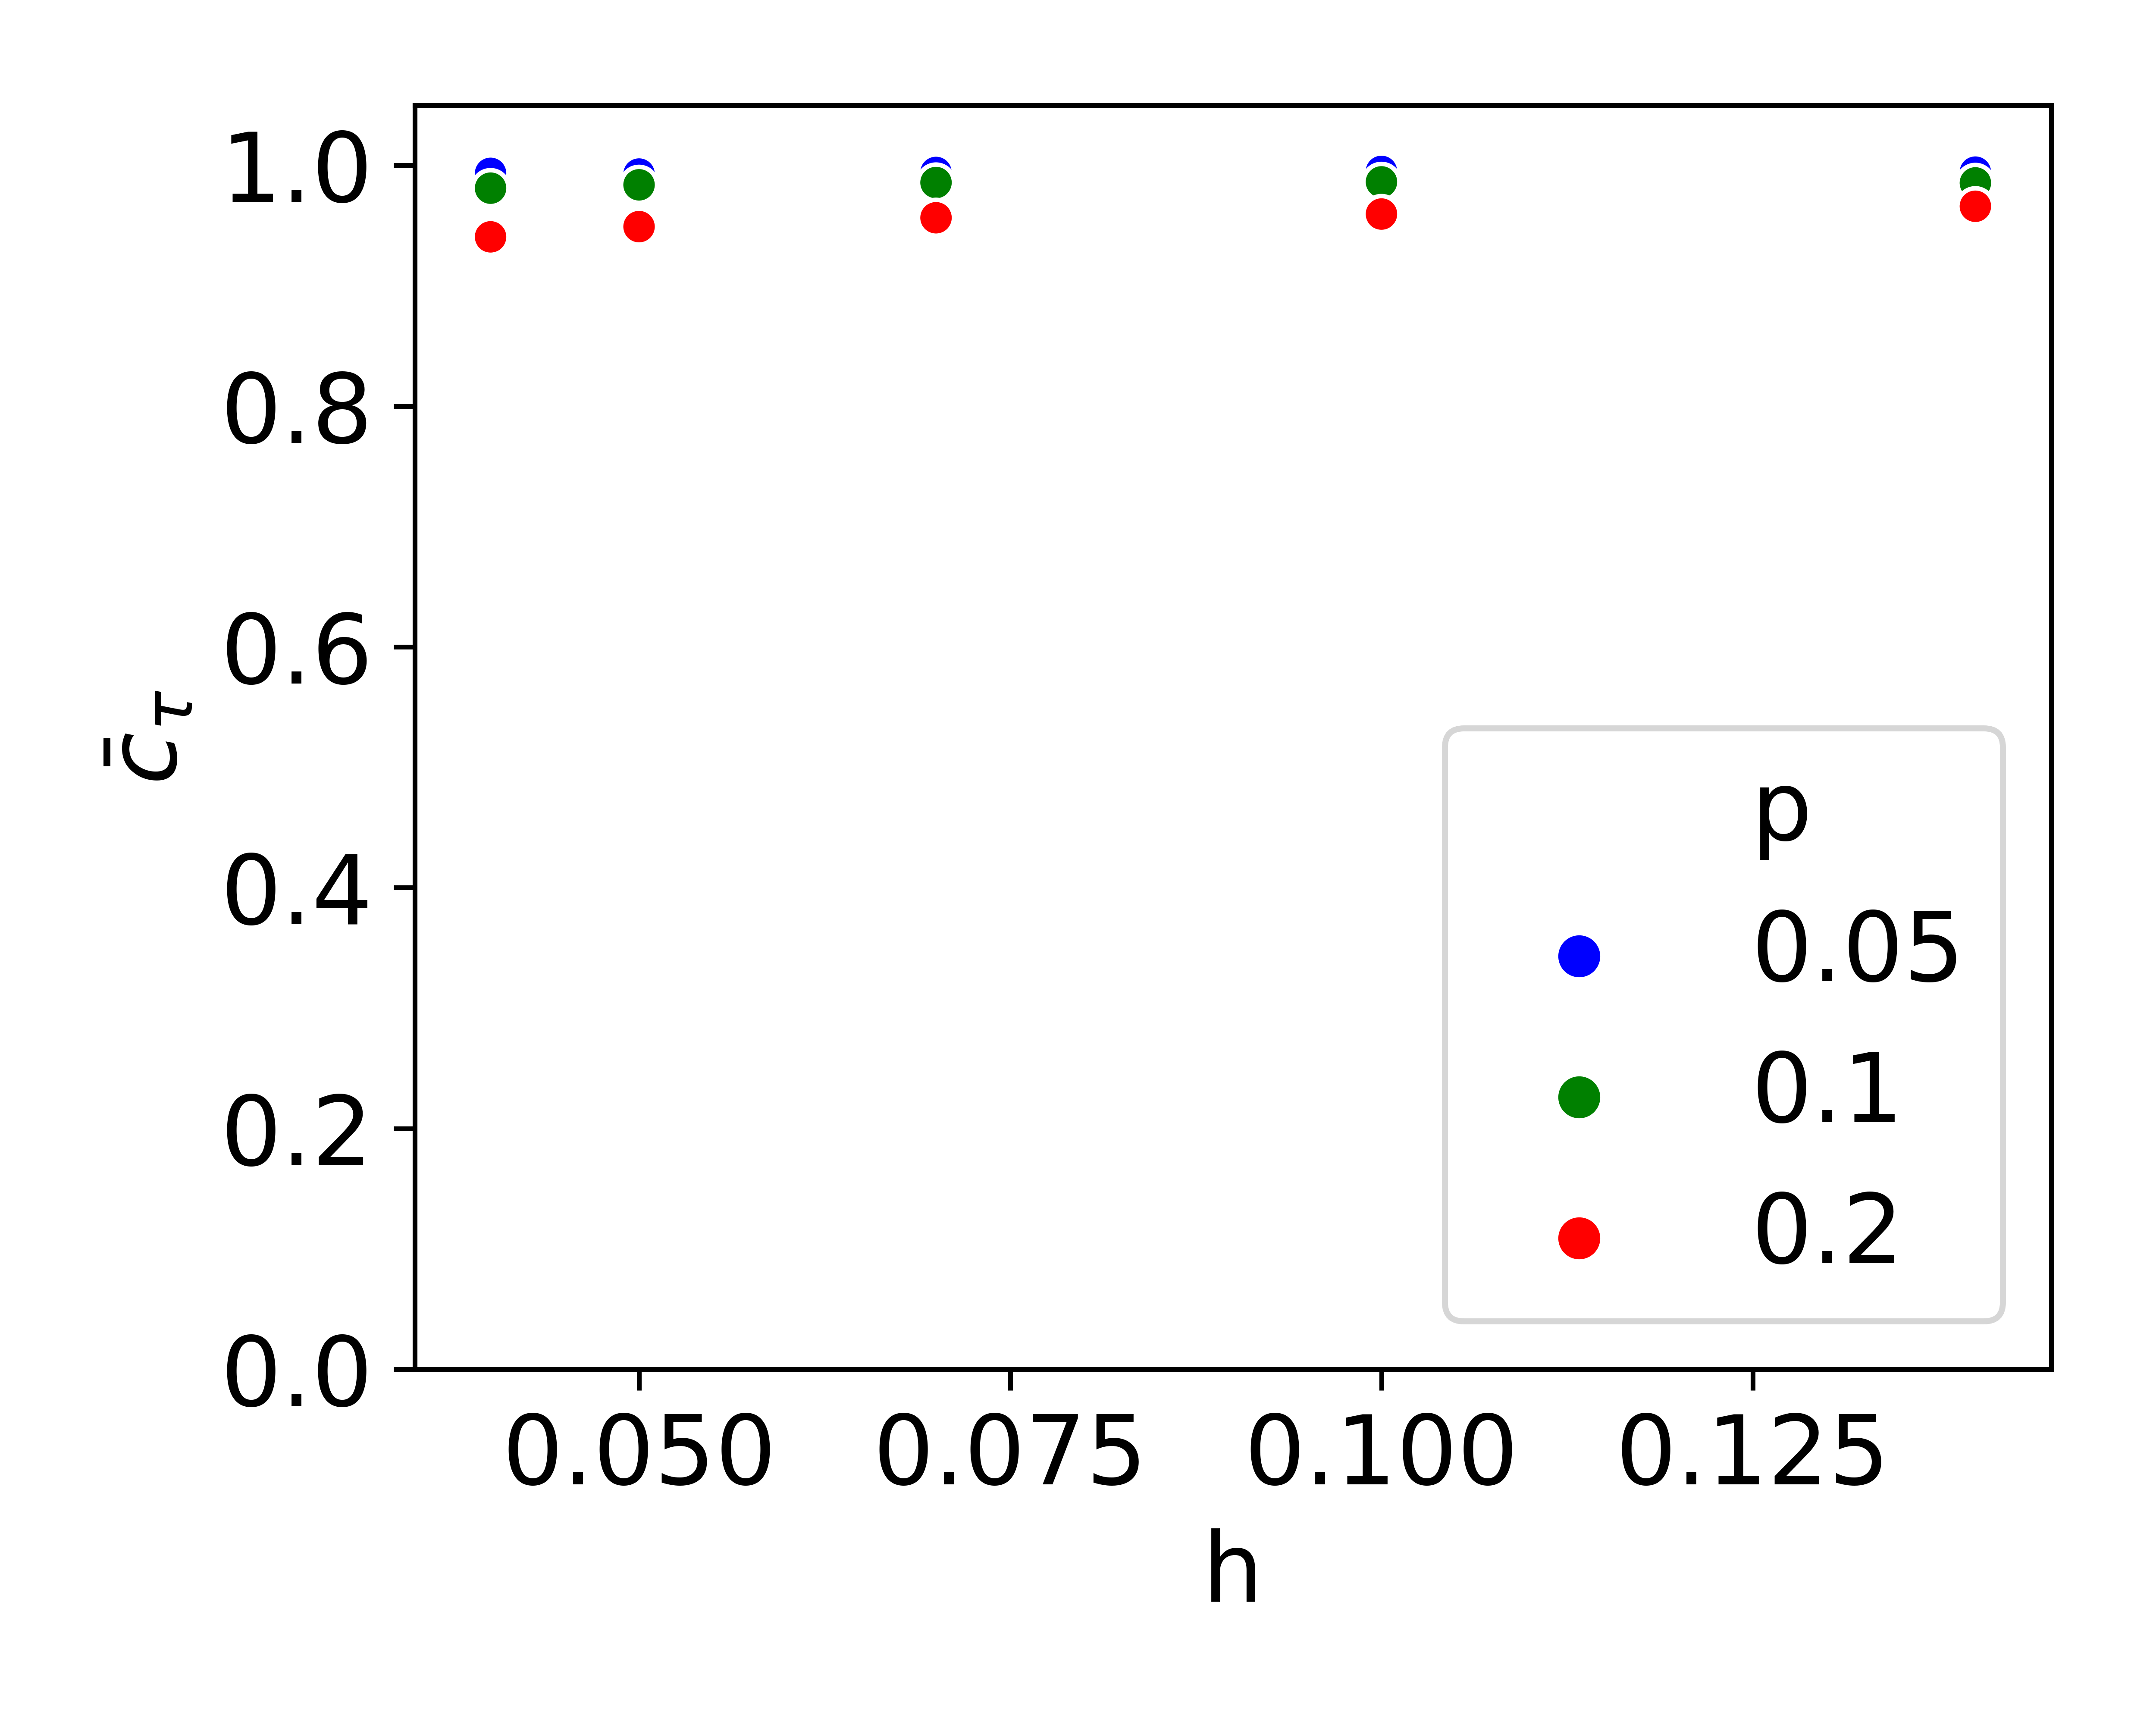
\includegraphics[width=0.7\textwidth]{../results/images/hp-watts-strogatz.png}
		\caption{Our work - simulation.}
	\end{figure}
\end{frame}

\begin{frame}{Barabasi-Albert results}
	\begin{figure}
		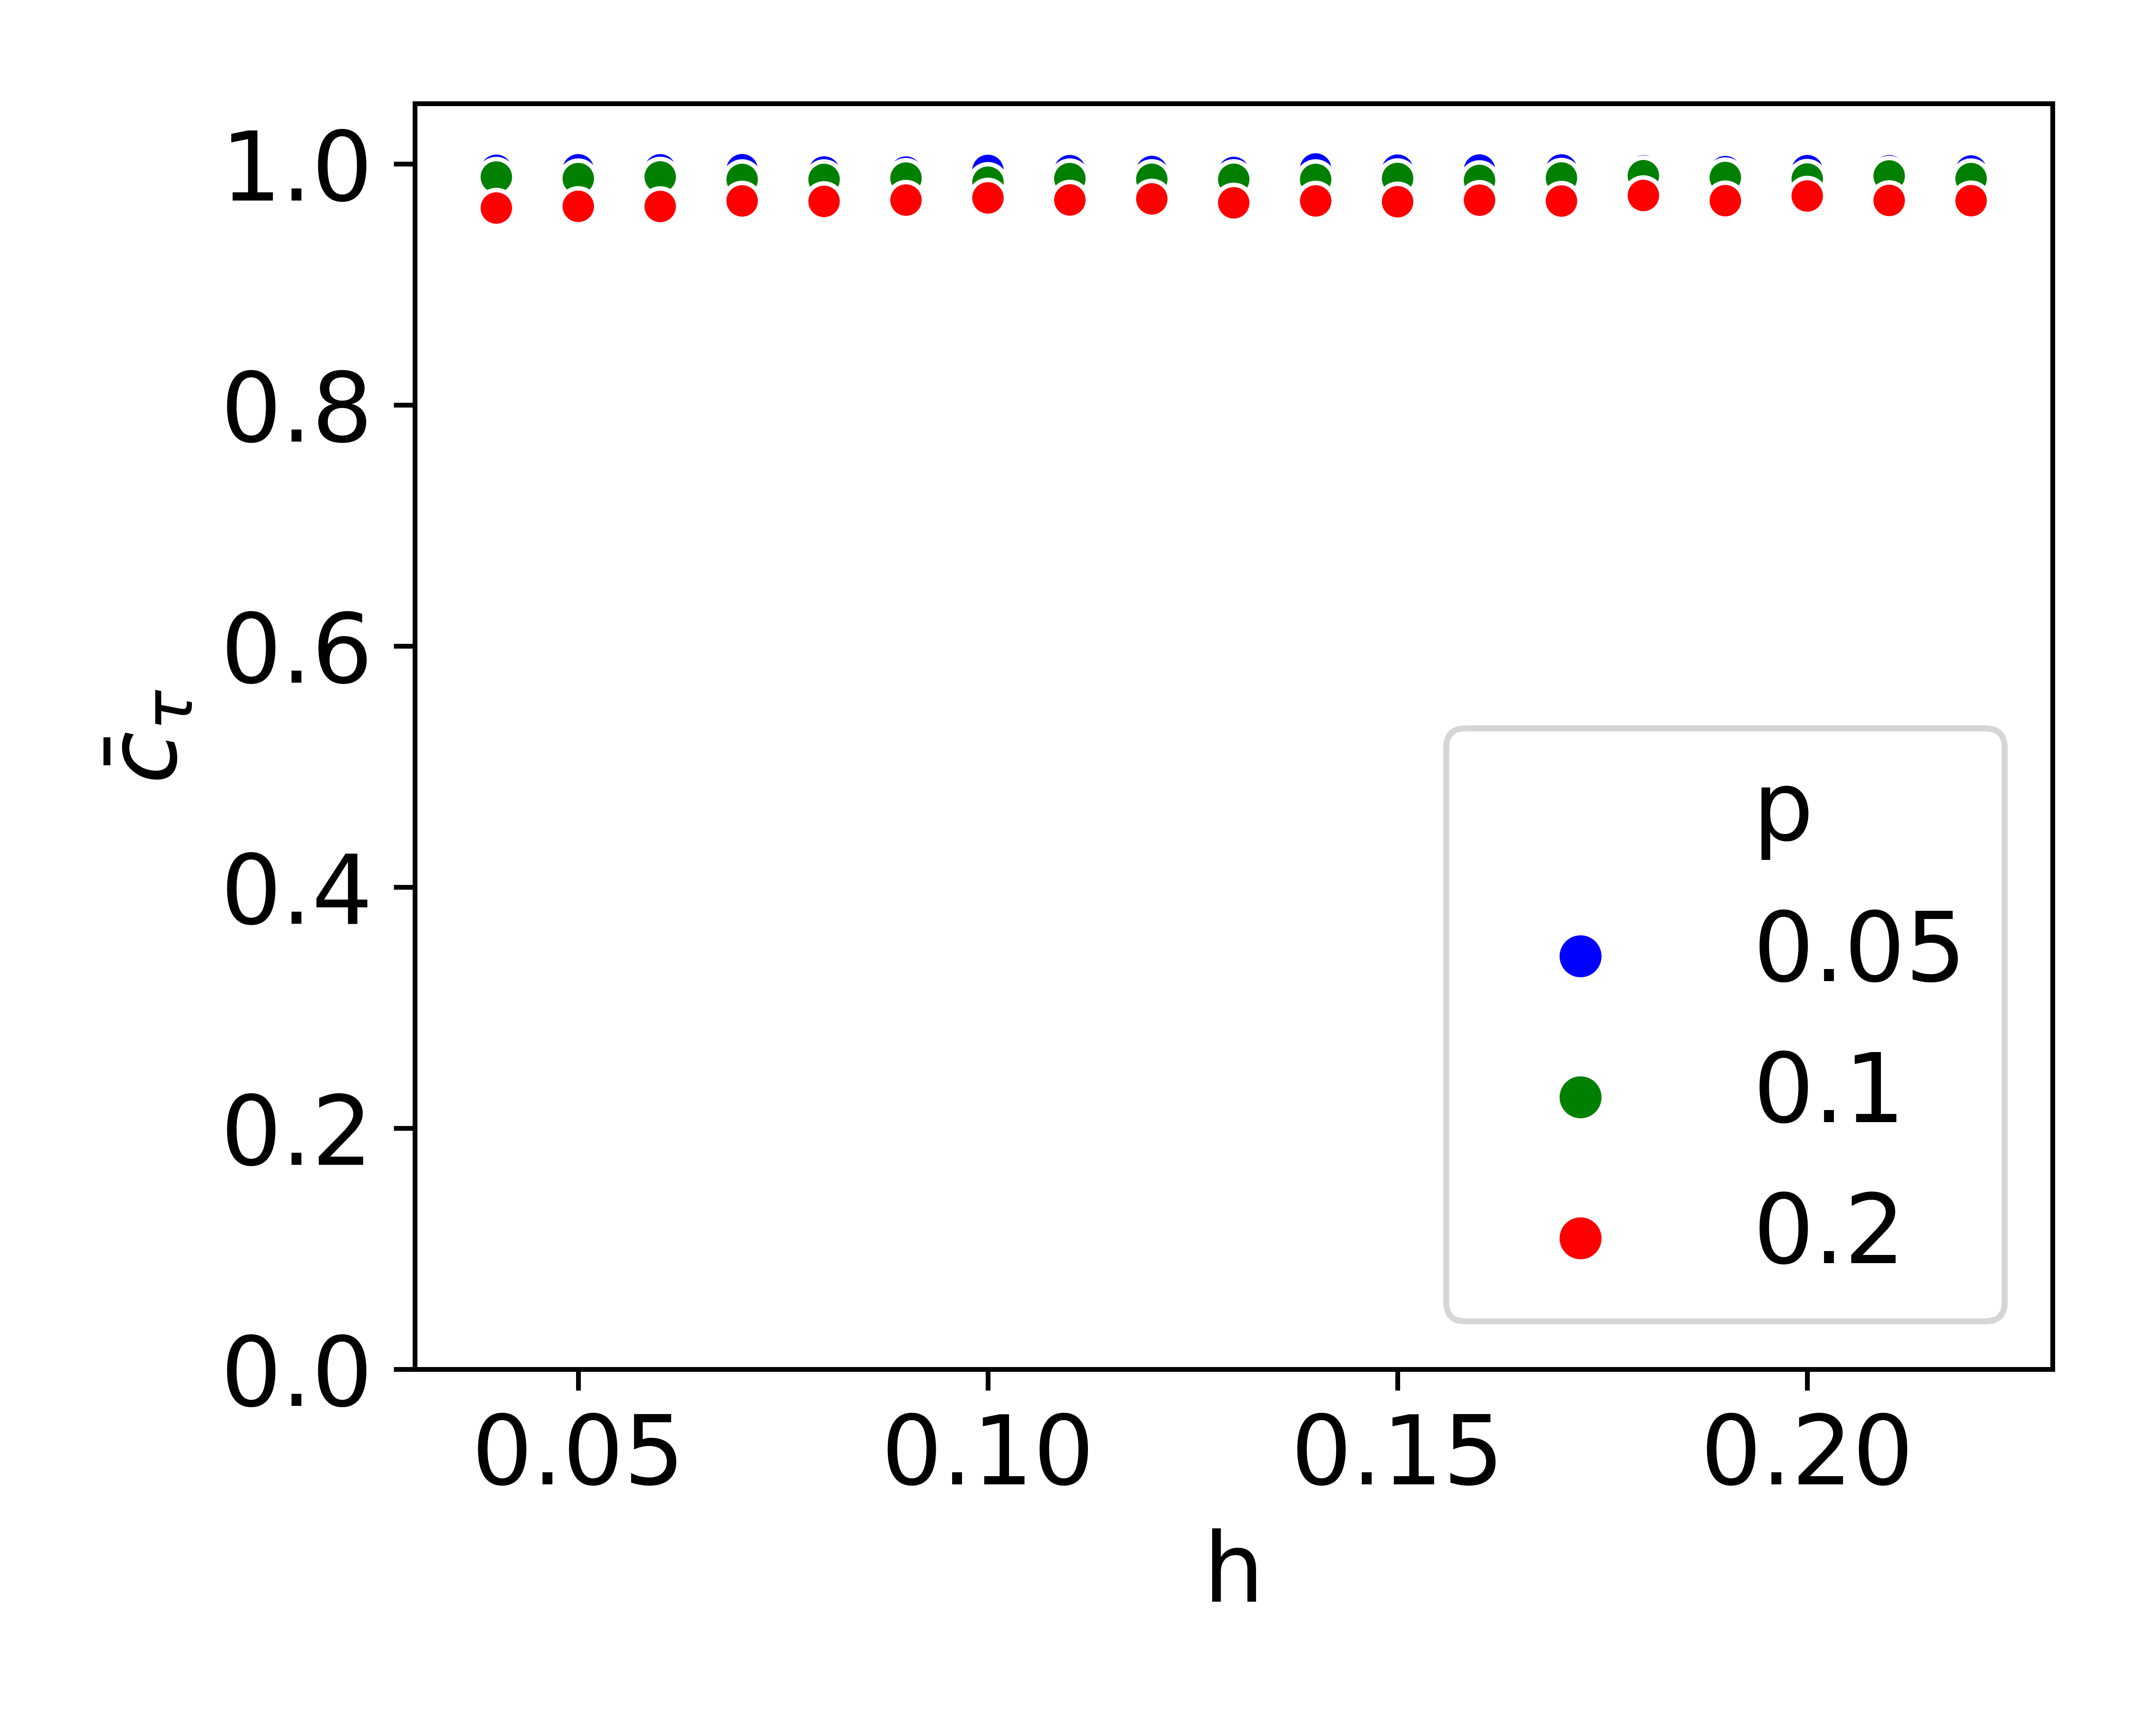
\includegraphics[width=0.7\textwidth]{../results/images/hp-barabasi-albert.png}
		\caption{Our work - simulation.}
	\end{figure}
\end{frame}

\begin{frame}{Comparison of models}
	
	Try to find universal $h$
	\begin{table}[]
		\begin{tabular}{l|llll}
			& \multicolumn{3}{c}{p} &  \\
			\hline
			Graph           & 0.05   & 0.1   & 0.2  &  \\
			\hline
			2D Lattice grid &        &       &      &  \\
			Complete graph  &        &       &      &  \\
			Watts-Strogatz  &        &       &      &  \\
			Barabasi-Albert &        &       &      & 
		\end{tabular}
	\end{table}
\end{frame}

\section{Conclusions}

\begin{frame}{Conclusions}
	\begin{itemize}
		\item Because of independence system never reaches an absorbing unanimous steady state.
		\item Independence allows to investigate the system in which initially there are no adopters.
		\item Differences between the article and our simulations may arise from the use of much smaller graphs.
	\end{itemize}
\end{frame}

\begin{frame}{Contributions}
	Presentation:
	\begin{itemize}
		\item Patryk Wielopolski
	\end{itemize}
	Plots and analysis:
	\begin{itemize}
		\item Maria Kowalczyk
		\item Anna Szymanek
	\end{itemize}
	Simulations:
	\begin{itemize}
		\item Patryk Wielopolski
	\end{itemize}
\end{frame}

\begin{frame}[allowframebreaks]{References}	
	\bibliography{references}
	\bibliographystyle{abbrv}
\end{frame}

\begin{frame}
	 \centering
	{\Large Thank you for your attention!}
	
\end{frame}

\end{document}
